\chapter{Stellar Activity Modelling in Radial Velocity Time Series}
As discussed in Sect.~\ref{sect:activity}, there exists a multitude of physical
processes ongoing within the photospheres and chromospheres of active stars
which produce observable signatures with a variety of amplitudes and timescales
(see Table~\ref{table:activity}). The subsequent sections discuss a variety of
techniques which have been used to model and consequently mitigate the effects of
stellar activity in RV time series.

\section{An Overview of Techniques for Stellar Activity Mitigation}
\label{sect:methods}

\subsection{Stellar Activity as a Scalar Parameter}
Back when the first giant exoplanets where being discovered with RVs,
typically a treatment of stellar activity was not implemented. The reason being
that the quality of the datasets at that time were insufficient to resolve the
temporal structure of RV activity for any but the most active stars. Many
observers however did report the root-mean-square (rms) of their RV residuals
following the removal of their best-fit planet model
\citep[e.g.][]{mayor95,butler96}. In
many cases this revealed residaul rms values which exceeded the characteristic RV
measurement uncertainty and thus alluded to the presence of additional
jitter signals which may or may not vary significantly with time. \\

In many of the following RV planet searches the apparent jitter was characterized
by an additive scalar $s$. The free parameter $s$ was used to characterize the
level of RV jitter as it was added in quadrature to the RV measurement
uncertainties when evaluating the objective function during any analysis
equivalent or analogous to a $\chi^2$-minimization routine. The nature of this
method assumes a fixed level of dispersion due to jitter that is constant in time.
As such, the resulting
measurement of $s$ does little more than inform us of the jitter amplitude as
any temporal evolution of activity, due to finite active region lifetimes or magnetic
cycles, will remain unresolved.

\subsection{Correlations with Activity Indicators}
Stellar RV observations are known to be affected by both planetary companions as
well as by stellar activity. Disentangling those signals in RV time series
therefore benefits significantly from ancillary time series which are sensitive
to stellar activity only \citep{boisse09}.
The classical implementation of de-correlation by
an activity indicator is to derive time series of one or many spectroscopic
activity indicators whose sampling is simultaneous with the RVs and then
fitting an often linear relation between those datasets (Fig.~\ref{fig:corr}) to
account for the temporal evolution of activity over the observational baseline.
The relation, when fitted simultaneously with planetary solutions, allows the RVs
to be de-correlated jointly with the measurement of the planetary parameters.
This technique has been shown to be effective when the stellar rotation period
\prot{} is well constrained, the planetary orbital period is distinct from
\prot{,} the amplitude of the planetary signal exceeds that of the activity signal
by $\gtrsim 30$\%, and the stellar rotation period is well sampled over multiple
cycles \citep{boisse11}. \\

\begin{figure}
  \centering
  %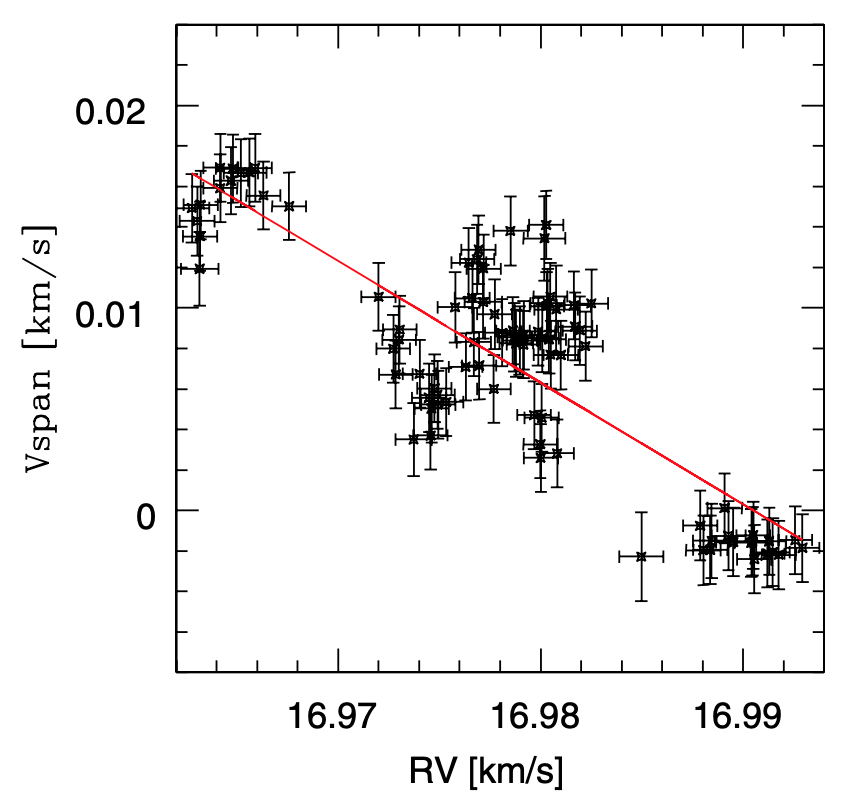
\includegraphics[width=.6\textwidth]{figures/vspan_rv.png}
  \caption[Correlation between stellar RVs and the \vspan{} activity indicator.]
      {The correlation of the \vspan{} activity indicator with the RVs for the
    active Sun-like star HD 17051 from HARPS spectra. The solid line depicts the
    best-fit linear relation from least squares fitting. The fitted relation is
    used to de-correlate the RVs for the effects of stellar activity as probed by
    the \vspan{} time series. \citep[Image credit:][]{boisse11}.}
  \label{fig:corr}
\end{figure}

There exists a number of activity indicators which can be derived from the stellar
spectra. There definitions and physical motivations are summarized below. \\

\emph{log R$'_{HK}$}:
the \caii{} H and K resonance lines are excited by non-thermal heating 
and act as a sensitive indicator of chromospheric structure and particularly of
the presence of bright chromospheric plages. 
For optical spectra with access to the \caii{} H and K lines
centered on 3968.47 \AA{} and 3933.66 \AA{,} the Mt. Wilson S-index is defined as

\begin{equation}
  \text{S-index} \propto \frac{\Psi_H + \Psi_K}{\Psi_B + \Psi_V}
\end{equation}

\noindent where $\Psi_H$ and $\Psi_K$ represent the narrowband
($\sim 1.1$ \AA{} wide) fluxes in the cores of the H and K lines of the \caii{}
doublet. The index is normalized by total flux in the $B$ and $V$ continuum bands
which are 20 \AA{} wide broad bands centered on 3900 and 4000 \AA{} respectively.
From this the \Rhk{} indicator is derived using a variety of formulations which are
all $\propto$ S-index and attempt to isolate the chromospheric component of
$\Psi_H$ and $\Psi_K$ from the photospheric component using normalization factors
which are dependent on \teff{} and level of stellar activity \citep{lovis11}. The
\Rhk{} indicator has been well characterized as a sensitive probe of activity on
both Sun-like stars and M dwarfs
\citep[e.g.][]{wright04,lovis11,astudillodefru17b}. \\

$H\alpha$: 
similarly to the \Rhk{} index, H$\alpha$ photons ($\lambda = 6562.81$ \AA{)} are emitted by
hot plages and thus act as a tracer of stellar activity originating from the chromosphere.
H$\alpha$ may act as a more suitable spectroscopic activity indicator for cool M dwarfs
which of lack significant flux in the \caii{} H and K lines \citep{robertson14}.
In practical terms,  
similar spectral features tracing a star's chromospheric structure may alternatively be used
as activity indicators depending on the accessible wavelengths of the employed spectrograph
(e.g. \hei{,} \nai{,} etc). \\


\emph{CCF shape parameters}:
the cross-correlation function (CCF) of a stellar spectrum represents its average line profile
at typically a high S/N.
As illustrated in Fig.~\ref{fig:starspot}, the presence of active regions distorts
the Gaussianity of the CCF thus alluding to the presence and nature of those active regions.
A number of shape parameters to the fitted CCF may be used to characterize stellar activity
using the same CCF from which the stellar RVs themselves are derived. However, these
spectroscopic diagnostics are only useful when they are robustly derived from high S/N
spectra of active stars where their effects on the CCF are clearly discernable \citep{desort07}.
Examples of three
shape parameters are visualized in Fig.~\ref{fig:ccf} and described below. \\

\begin{figure}
  \centering
  %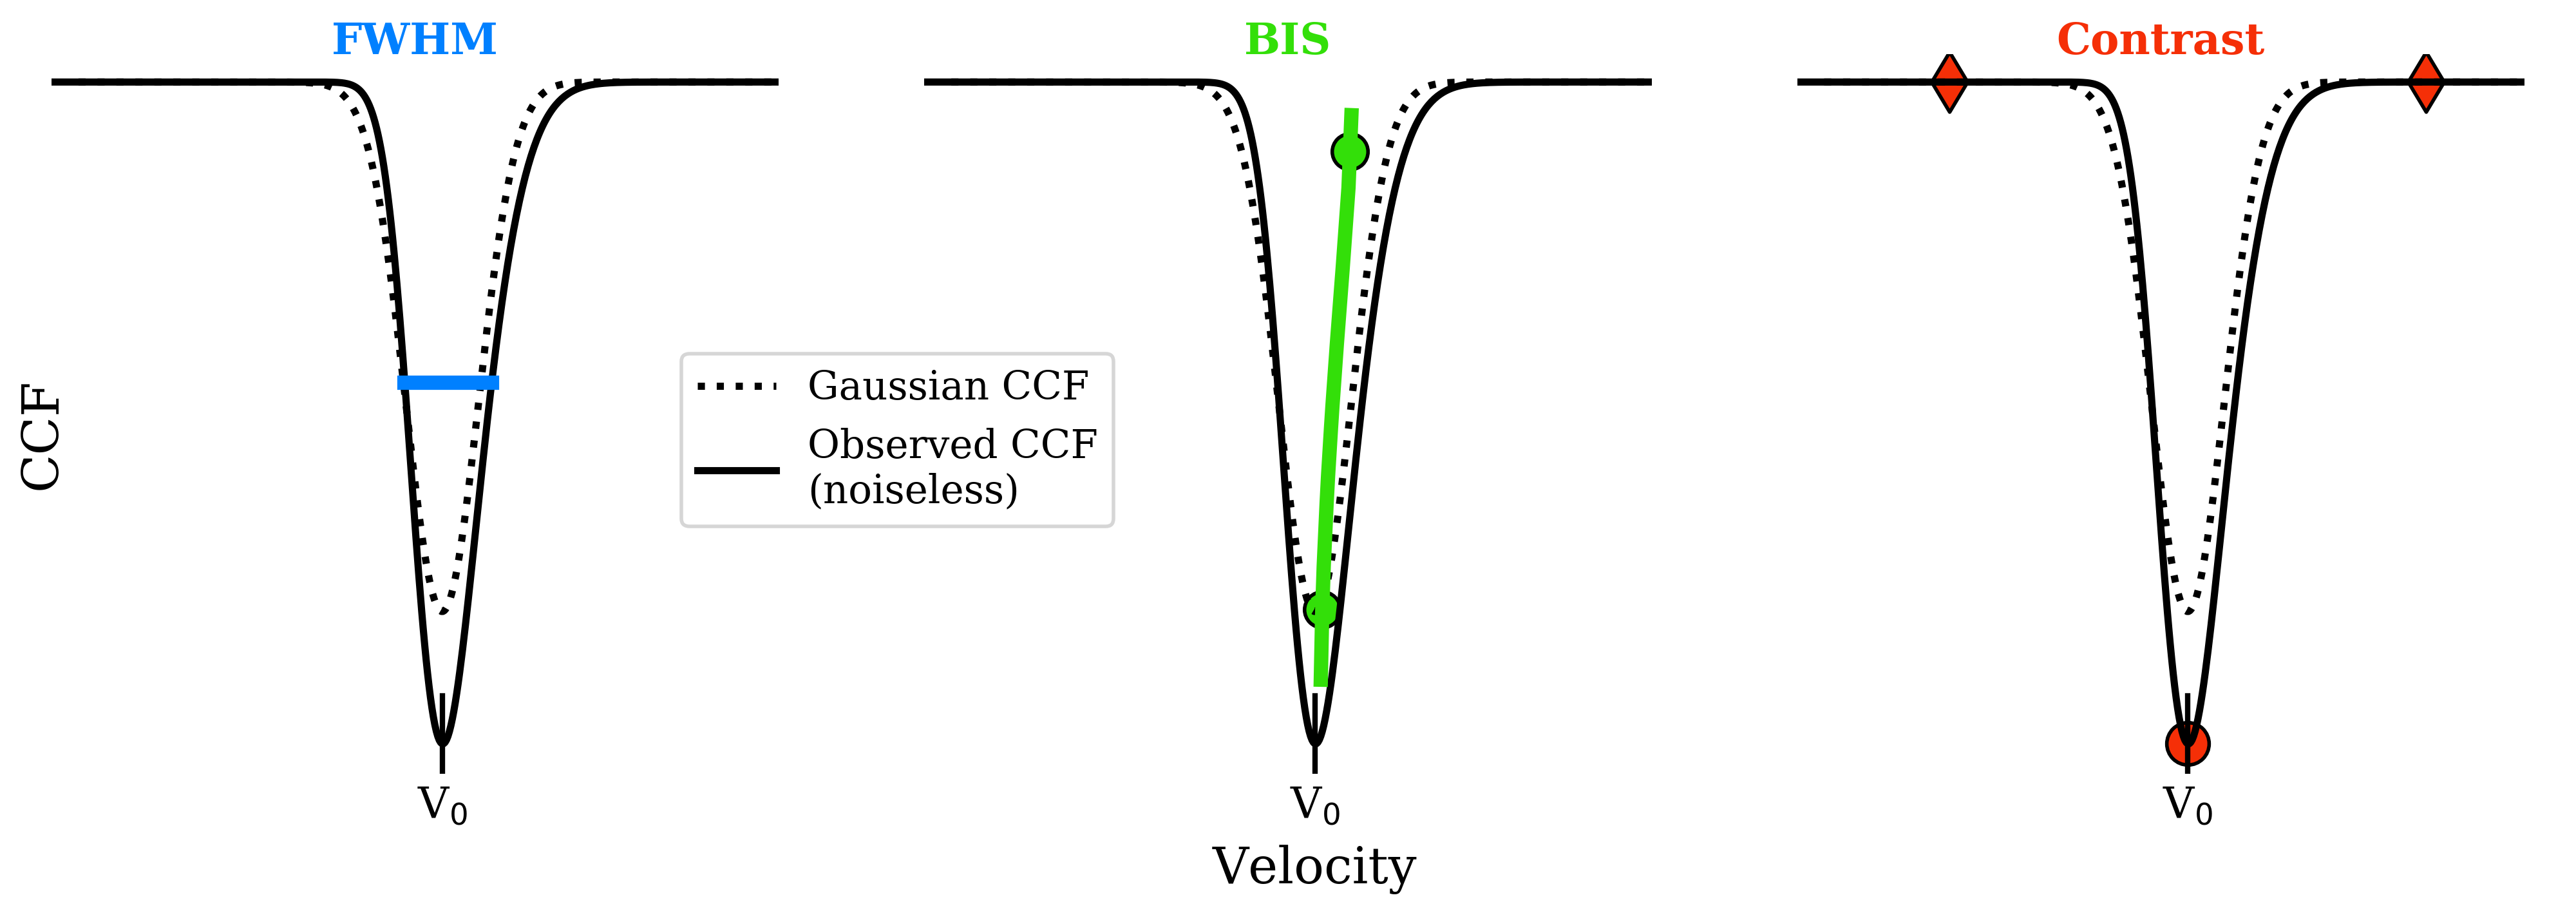
\includegraphics[width=\hsize]{figures/ccf.png}
  \caption[Illustrations of CCF shape parameters.]
          {Illustrations of measurements of the CCF width, asymmetry, and contrast via the full
            width half maximum (FWHM), bisector (BIS), and contrast shape parameters. The FWHM
            characterizes broadening of the CCF due to active regions at unique velocities on the
            stellar disk. The
            BIS characterizes the asymmetry of the line profile by computing the difference in
            average velocity in the upper and lower portions of the CCF (green circles in the
            middle panel). The contrast characterizes the depth of the CCF by taking the average
            of the CCF in the contiuum (diamonds) and its difference with the CCF flux at the
            stellar velocity $V_0$.}
  \label{fig:ccf}
\end{figure}

\emph{FWHM}:
the full width half maximum (FWHM) of the CCF is commonly used as a measure of CCF
width. As an active region transverses the rotating stellar disk across the differentially
Doppler-shifted limbs, its temperature contrast with the stellar photosphere adds additional
power to the CCF in the velocity direction opposite the occulted limb. This results in a
broadening of the CCF on one side of its mean velocity $V_0$. As illustrated in
the first panel in Fig.~\ref{fig:ccf},
the FWHM can be measured from the width of the CCF at a specified location. \\

\emph{BIS}:
recall that the broadening of the CCF due to a single active region is asymmetric about $V_0$.
A common shape parameter to characterize the resulting asymmetry is the bisector
\citep[BIS;][]{queloz01}.
Similar parameters have also been proposed as measures of CCF asymmetry such as the curvature of
the bisector line \citep{hatzes96}, the velocity span \citep{boisse11}, and the BIS inverse
slope \citep{queloz01}. Their definitions are closely related and rely on computing the weighted
velocity in the upper and lower portions of the CCF (see middle panel of Fig.~\ref{fig:ccf})
and computing their difference. A symmetric line profile will therefore have a BIS$=0$ whereas
asymmetric profiles affected by active regions will be non-zero and whose exact value and units
will depend on the defintion of the asymmetry parameter used. \\

\emph{Contrast}:
\citep{boisse09} noted that increasingly active stars, based on their fractional coverage by dark
star spots, tend to have shallower line profiles. This is the direct result of such stars featuring
greater contributions to their average line profiles from cool and therefore dimmer regions.
This effect is often characterized by the CCF contrast which is equal to the difference between the
average baseline of the CCF in the continuum (located many standard deviations away from $V_0$ in
the CCF wings) and the flux at the stellar velocity $V_0$.


\subsection{Photometric Modelling: the \textbf{\emph{FF}}$'$ Method} \label{sect:ffp}
An alternative to using simultaneous spectroscopic activity indiciators to temproally de-correlated
RV measurements for the effects of stellar activity, \citep{aigrain12} present the $FF'$ formalism
which uses contemporaneous photometry to model two distinct RV activity components. \cite{aigrain12}
argue that in the limit of small active regions with non-complex configurations, the fractional
coverage of the stellar disk by active regions (i.e. spots) $F(t)$ is related to the photometric flux
$\Psi(t)$ via

\begin{equation}
  \Psi(t) = 1 - F(t).
  \label{eq:ffp}
\end{equation}

\noindent Eq.~\ref{eq:ffp} reads that the fractional spot coverage is just one minus the observed
stellar flux in normalized units such that the star's brightness equals unity in the absence of spots.
The corresponding RV signals from a active regions giving rise to the photometric variations are known
as the rotation or flux effect $\Delta \text{RV}_{\text{rot}}$ and the convection blueshift effect
$\Delta \text{RV}_{\text{conv}}$. The former arises from active regions occulting the differentially
Doppler-shifted stellar limbs and thereby suppressing the flux of photons with a particular
Doppler-shift. Because the rotation effect affects the RVs in proportion to the spot coverage and
exhibits a sign change as the spot crosses from the blueshifted limb to the redshifted limb over a single
rotation cycle, the rotation effect is

\begin{equation}
  \Delta \text{RV}_{\text{rot}}(t) \propto F(t) \dot{F}(t)
\end{equation}

\indent where the first time derivative of the fractional active region coverage is
$\dot{F}(t) = -\dot{\Psi}(t)$ from Eq.~\ref{eq:ffp}. As such, the rotation effect tends to dominate
on rapidly rotating stars wherein $\dot{F}(t)$ is large. Conversely, the convective blueshift effect
operates by active regions disrupting the homogeneity of the stellar disk on which convective
blueshift is on-going everywhere. This disruption scales with the fractional spot coverage and
the angle between the spot normal and the line-of-sight which results in

\begin{equation}
  \Delta \text{RV}_{\text{conv}}(t) \propto F^2(t).
\end{equation}

\noindent The convective blueshift effect tends to dominate more slowly rotating spotted
stars such as the Sun \citep{haywood16}. \\

Fig.~\ref{fig:ffp} demonstrates both the rotation and
convective blueshift effects on the RVs and how they are related to the photometric detriment
incurred by a single spot over a portion of one stellar rotation cycle.

\begin{figure}
  \centering
  %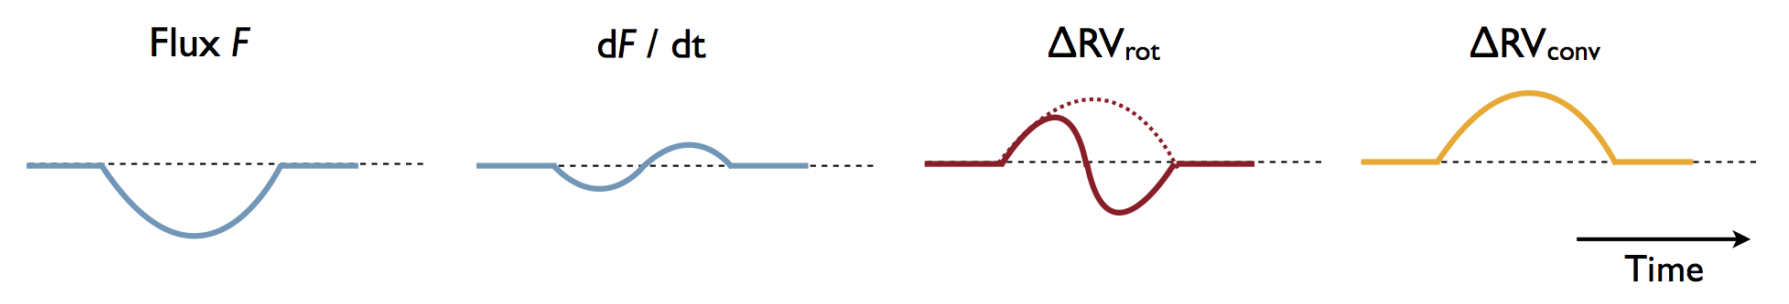
\includegraphics[width=0.8\hsize]{figures/ffp.png}
  \caption[Illustration of the $FF'$ method.]
      {The $FF'$ method for deriving the rotation and convective blueshift components
    of stellar RV activity from contemporaneous photometry. Here the photometric stellar flux
    is used to infer the fractional spot coverage $F(t)$. The rotation effect scales with
    $F(t) \dot{F}(t)$ and thus varies with half the period as does the convective blueshift
    effect which scales as $F^2(t)$. \citep[Image credit:][]{haywood15}.}
  \label{fig:ffp}
\end{figure}


\subsection{Pre-whitening}
This method aims at identifying strong periodicities in the RV time series and removing also
such signals until only residual Gaussian noise is remaining. This method known as pre-whitening
is based on analyzes of multi-periodic stellar oscillation modes and works by performing a Fourier
transform of the data and removing sinusoidal functions from the raw data whose periods and
identified by the frequency analysis \citep{queloz09}. Pre-whitening assumes that all signals
are long-lived and sinusoidal which is not always applicable for the stellar activity signals
that it aims to mitigate. 

\subsection{Deterministic Model Fitting}
RV time series exhibiting strong coherent signals at either \prot{} or its first
harmonic\footnote{As can be the case for rapidly rotating spotted stars whose RV activity
  is dominated by the rotation effect (see Sect.~\ref{sect:ffp}).} may be well modelled by
a deterministic function in the form of a sinusoid at \prot{} or $P_{\text{rot}}/2$
\citep{boisse11}. In general, such models are incomplete because they neglect any temporal
evolution of active regions which vary in their sizes, temperatures, and spatial distributions
over adjacent rotation cycles \citep{giles17}. These nuances are not captured in a 
deterministic sinusoidal model although this methodology may still be applicable in time series
with short observational baselines or for stars with long-lived active region groups.


%\subsection{Physical Models of Active Regions}
%\citep{dumusque14}


%\subsection{Spectral Feature Decomposition}
\subsection{Line by line radial velocities}
Spectral lines are known to be affected differently by stellar activity due to their
sensitivities to pressure, temperature, embedded magnetic field strength, and fluid
velocity which are all affected by stellar activity \citep{davis17,wise18}. These
effects from stellar activity to spectral line shapes are distinct from Doppler-induced
line shifts which are identical to all lines. \cite{dumusque18} investigated
the prospect of deriving stellar RVs line by line. The resulting RVs derived from
individual lines were shown to be
consistent with the archival RVs derived from the HARPS data reduction software.
The derivation of RVs in this way is postulated to mitigate anomalous RV signals
from stellar activity if spectral features that are minimally affected by activity
are utilized. Intelligent identification of lines that are minimally sensitive to
activity remains an active area of research. \\

\cite{davis17} also demonstrated the power of analyzing individual spectral lines
to identify the effect of stellar activity on RVs. Principal component analysis
is run on sets of idealized spectra from stars containing either an equatorial spot,
an equatorial facula, or a planetary companion on a circular orbit. As shown in
Fig.~\ref{fig:pca}, the maximum variance contained in the first principal component
of the Doppler-shifted spectrum (i.e. with no activity) is maximized where the slope
of spectral features is greatest and is identical to all spectral features as they
are each equivalently affected by Doppler shifts. Lines in the remaining synthetic
spectra that are affected by either a spot or facula or not identically affected due
to the differential sensitivity of various lines to their physical environments
which in turn are influenced by the presence of active regions. Fig.~\ref{fig:pca}
reveals examples of strongly varying lines from Ti \footnotesize I \normalsize and Ni
\footnotesize I \normalsize at 5009.5 \AA{} and 5010.8 \AA{} respectively.
\cite{davis17} also quantify the wealth of information contained in the spectra
as a function of S/N and spectral resolution and argue for the need to obtain
high resolution spectra to finely resolve line profiles and exploit their inherent
activity information content.

\begin{figure}
  \centering
  %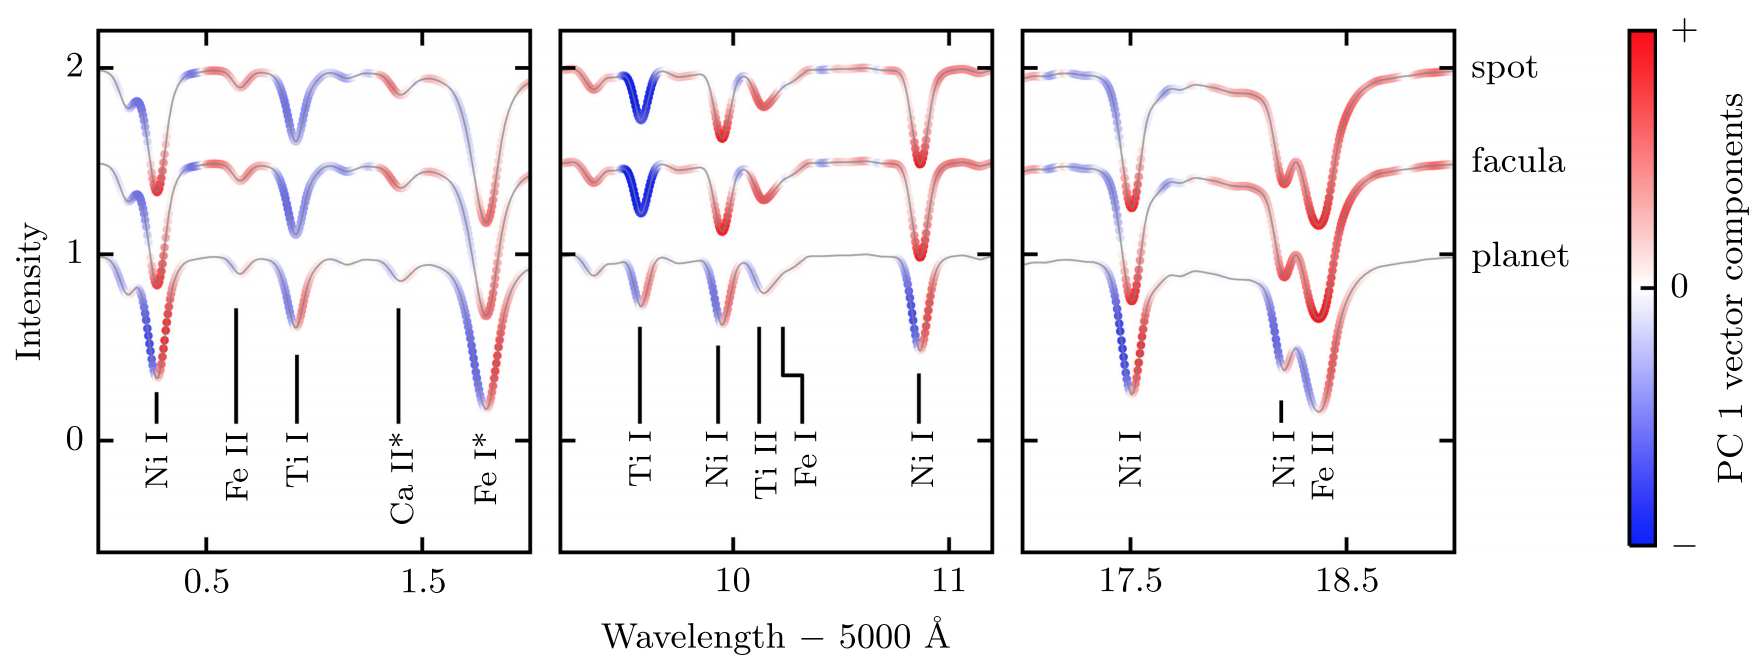
\includegraphics[width=\hsize]{figures/pca.png}
  \caption[Principal component analysis of idealized spectra containing either spots, faculae, or planets.]
          {The values of the first principal component for three spectra of a star with either an equatorial
            spot, an equatorial facula, or a circular keplerian orbit. The maximum variance (with either sign)
            in the Doppler-shifted spectrum is dominated by regions with the greatest slope and is the same
            for all spectral features. Variance in the active spectra and not equal within each line as not all
            lines respond identically to in the presence of active regions. \citep[Image credit:][]{davis17}}
  \label{fig:pca}
\end{figure}


\section{Gaussian Process Regression for Non-Parametric Activity Modelling} \label{sect:gp}
Many of the shortcomings of the activity mitigation techniques discussed in the
previous sections are based on their incompleteness and their inability to
self-consistently characterize model uncertainties. For example, correlations with
activity-sensitive time series are often incomplete because the chosen indicator
is not sensitive to also activity sources present in the RVs and often result in
large RV residuals after de-correlation. Similarly, deterministic activity models
lack sensitivity to stochastic changes in activity levels due to the evolution
of active regions between adjacent rotation cycles or over
significant subsets of long-term magnetic cycles. \\

Gaussian process regression models represent one such tool which aims to overcome
these shortcomings by jointly modelling planets and activity in a self-consistent
manner. This technique originally pioneered on active Sun-like stars
\citep[e.g.][]{haywood14,grunblatt15,faria16,lopezmorales16}
has been shown to reconcile disparate solutions
between observations from multiple spectrographs \citep{rajpaul17,cloutier19},
to reconcile RV solutions for planetary systems whose favoured models are
ambiguous \citep{rajpaul17,cloutier19}, and to disentangle neighbouring periodic
signals from planets, stellar rotation, and/or from window functions
\citep{rajpaul16,cloutier17b}.
In the following sections I will give an overview
of what Gaussian processes are and how I implement their formalism in the context
of modelling stellar activity in RV time series.

\subsection{The one dimensional Gaussian distribution}
A Gaussian process (GP) is defined as \emph{a collection of random variables, any
finite subset of which has a joint Gaussian distribution}. In other words,
any random process\footnote{A random process is any collection of random
  variables indexed by an independent variable such as time.} for which all
finite subsets have a multivariate Gaussian distribution, is a Gaussian process
\citep{rasmussen05}. 
In order to develop a visual intuition of the definition of a Gaussian process,
let us a first consider a Gaussian random variable in one dimension. \\

Imagine some random
process that draws a single value of a random variable $X$ for each realization of
an experiment. As an astronomer with a life
outside of astronomy, and furthermore as an astronomer who spends many of his
off-work hours being pelted with %170 gram
disks of vulcanized rubber, my favourite
Gaussian random variable has to be the `goals against average' statistic:

\begin{equation}
  X = GAA \equiv \frac{\text{total number of goals against}}{\text{total number of games played}}.
\end{equation}

\noindent As a Gaussian random variable, the results of repeated experiments (i.e.
repeated draws from the empirical $GAA$ distribution for various goaltenders) can
be expressed by the Gaussian probability density function (PDF) of the form

\begin{equation}
  \mathcal{N}(X|\mu,\sigma^2) = \frac{1}{\sqrt{2\pi \sigma^2}} \exp{\left(
    -\frac{(X-\mu)^2}{2\sigma^2} \right)},
  \label{eq:gauss}
\end{equation}

\noindent which is parameterized by $\mu=\text{mean}(X)$ and $\sigma^2=\text{var}(X)$;
i.e. the mean and variance of $X$. As shown in Fig.~\ref{fig:gaa1d}, the empirical
distribution of the $GAA$ for goaltenders in
the National Hockey League (NHL) over the past five seasons closely follows a
Gaussian distribution with a mean of 2.64 and a standard deviation of 0.40 goals
against per game. Hence, my favourite Gaussian random variable. \\

\begin{figure}
  \centering
  %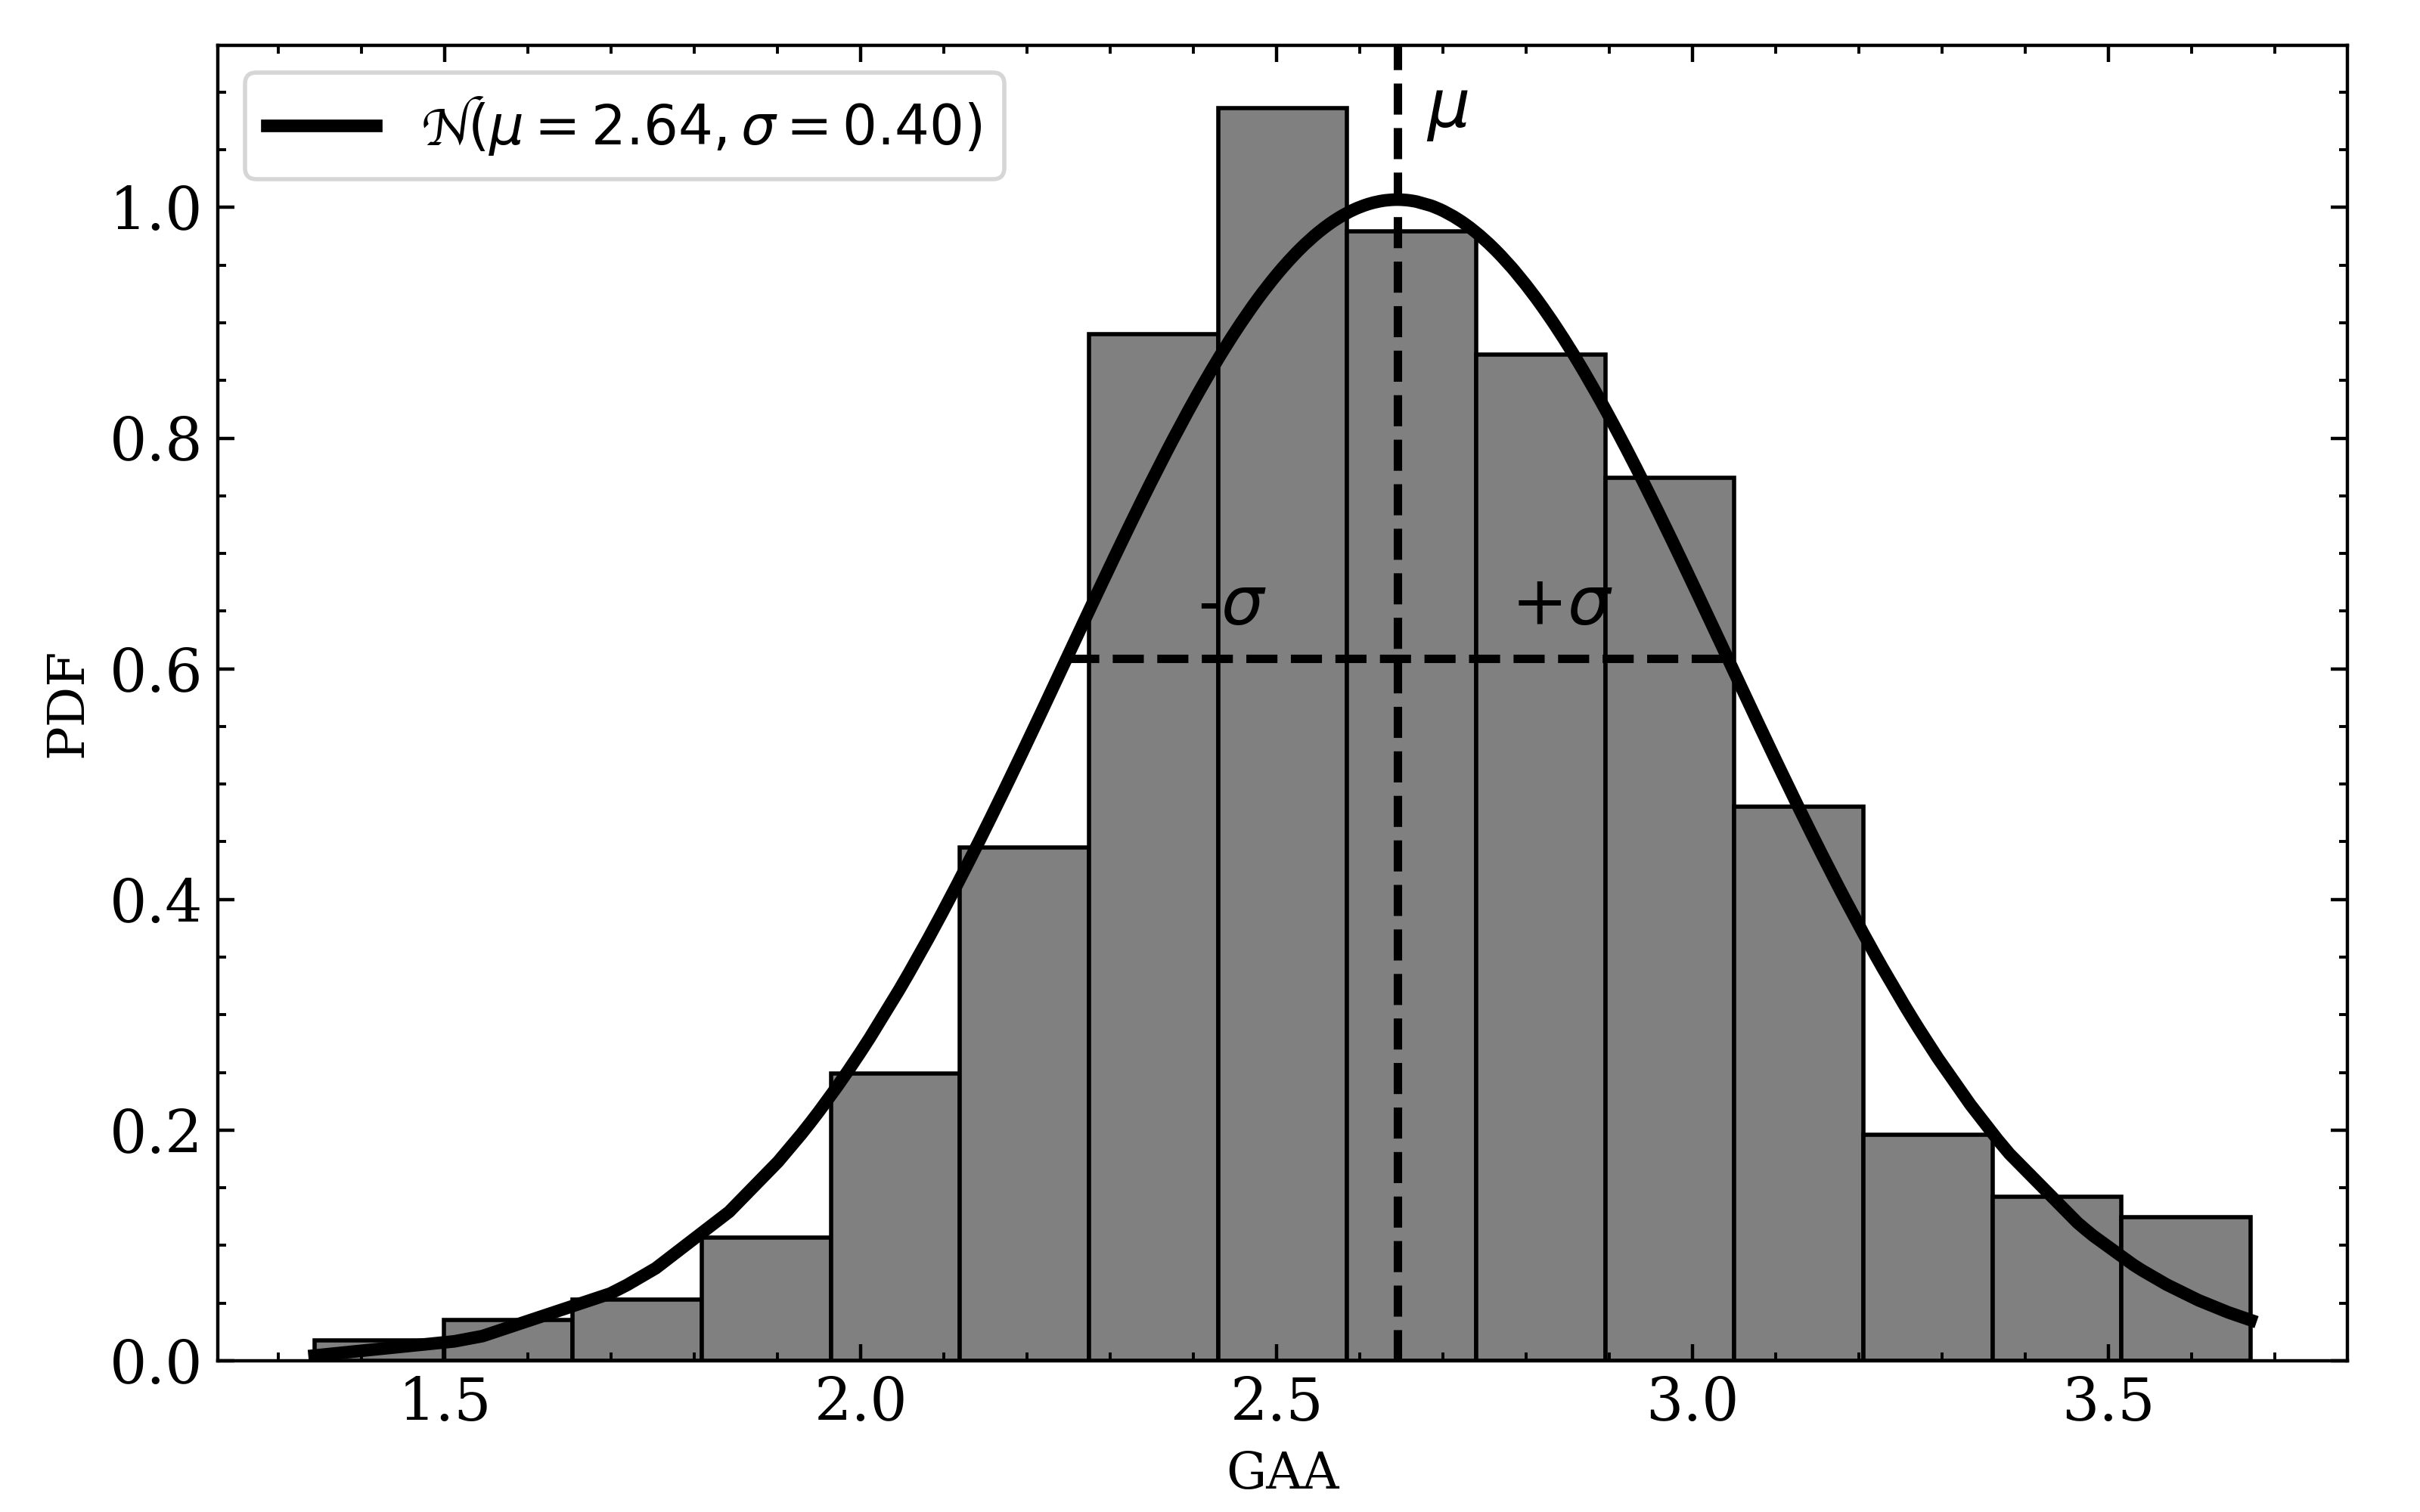
\includegraphics[width=.8\textwidth]{figures/GAA1D.png}
  \caption[Gaussian random variable in one dimension.]
      {The distribution of $GAA$ for NHL goaltenders over the past five
    seasons as an example of a Gaussian random variable. The solid line depicts
    the Gaussian probability density function with mean and standard
    deviation 2.64 and 0.40 goals against per game.}
  \label{fig:gaa1d}
\end{figure}

Before a new season begins, we can write down a prior distribution on the $GAA$
based on the prior knowledge we have obtained from previous NHL seasons; i.e.
$\mathcal{N}(GAA|2.64,0.16)$. This distribution has a unique expection value and
variance describing what we expect any given goaltender's $GAA$ to be in an
up-coming season and, as crucially, how precisely that value constrained.

\subsection{The two dimensional Gaussian distribution}
Of course we can introduce a second Gaussian random variable and extend the 
concept of the one dimensional Gaussian distribution to two dimensions. This is done
by recasting the expression for the Gaussian PDF in $k>1$
dimensions where $k=2$ in this scenario. Rewriting Eq.~\ref{eq:gauss} in $k$
dimensions is achieved by replacing the scalar mean and variance with a mean
$k$-vector $\boldsymbol{\mu}$ and a $k \times k$ covariance matrix $\mathbf{K}$
respectively. The updated expression for the so-called multivariate Gaussian
distribution in $k$ dimensions is

\begin{equation}
  \mathcal{N}(\mathbf{X}|\boldsymbol{\mu},\mathbf{K}) = \frac{1}{\sqrt{(2\pi)^k
      |\mathbf{K}|}} \exp{\left( -\frac{1}{2} (\mathbf{X} -
    \boldsymbol{\mu})^{\text{T}} \mathbf{K}^{-1} (\mathbf{X}-\boldsymbol{\mu})
    \right)}.
  \label{eq:gauss2d}
\end{equation}

\noindent The $k$-vector $\boldsymbol{\mu}$ represents the mean value of each
random variable in $\mathbf{X}=(X_1,\dots,X_k)^{\text{T}}$.
The elements of the covariance matrix
$\mathbf{K}$ represent the covariances between each pair of random variables.
The diagonal elements of $\mathbf{K}$ therefore represent the covariance of each
random variable with itself, or equivalently the variance of that random variable.
The covariance between two random variables $X_1$ and $X_2$ can be computed explicitly
in terms of their expectation values E[$X_1$] and E[$X_2$] via

\begin{align}
  \text{cov}(X_1X_2) &= \text{E}[(X_1-\text{E}[X_1]) - (X_2-\text{E}[X_2])] \\
  &= \text{E}[X_1X_2] - \text{E}[X_1]\text{E}[X_2].
  \label{eq:coveq}
\end{align}

\noindent Note that the expectation value of a Gaussian random variable is simply
its mean. \\

\subsubsection{Uncorrelated variables}
Consider the special case of when the two Gaussian random variables under
consideration $X_1$ and $X_2$ are uncorrelated; i.e. cov$(X_1X_2)=0$. A quick
example of this is to let $X_1=GAA$ and sample $X_2$ from a independent Gaussian
distribution with zero mean and unit variance.
The nature of sampling $X_2$ in this way ensures
that $X_1$ and $X_2$ are indeed uncorrelated. The corresponding covariance matrix

\begin{equation}
  \mathbf{K}(GAA,X_2) =
  \begin{bmatrix}
    0.15 & 0.00 \\
    0.00 & 0.98
  \end{bmatrix}
  \label{eq:Kuncorr}
\end{equation}

\noindent is calculated using Eq.~\ref{eq:coveq} is diagonal and confirms that
$X_1$ and $X_2$ are uncorrelated as the off-diagonal elements of $\mathbf{K}$ are zero.
This fact can also be seen in the joint $X_1X_2$ distribution in Fig.~\ref{fig:uncorr2d}.
Because the variables $X_1$ and $X_2$ are uncorrelated in this example the
measurement of a value of $X_1$ does nothing to inform us of its corresponding
$X_2$ value. That is that the prior distribution
$\mathcal{N}(\mathbf{X}|\boldsymbol{\mu},\mathbf{K})$ is uninformative with regards to
$X_2$ in a sample for which the corresponding value of $X_1$ is known. \\

\begin{figure}
  \centering
  %\includegraphics[width=.9\textwidth]{figures/uncorr_2d.png}
  \caption[Uncorrelated Gaussian random variables in two dimensions.]
      {The one and two dimensional distributions of the Gaussian random
        variables $GAA$ and draws from the standard normal disribution (i.e. $\mathcal{N}(0,1)$).
        The solid
    lines overlaid on their joint distribution represent the 1, 2, and 3$\sigma$
    contours. The covariance matrix (Eq.~\ref{eq:Kuncorr}) has off-diagonal
    elements equal to zero indicating that the two variables are uncorrelated;
    a property which is largely discernable from the lack of correlation in their joint
    distribution.}
  \label{fig:uncorr2d}
\end{figure}

\subsubsection{Correlated variables}
But what if next we consider an alternate Gaussian random variable. Namely
$X_2 = SV$\% where

\begin{equation}
  SV\% \equiv \frac{\text{total number of saves made}}{\text{total number of shots faced}}
\end{equation}

\noindent is a measure of a goaltender's save percentage. In this scenario one
might expect the variables $GAA$ and $SV$\% to have some degree of correlation
as a ``good'' goaltender who boasts a low $GAA$ probably does so because of their
high $SV$\%. Indeed the covariance matrix of the $GAA$ and $SV$\% for NHL
goaltenders over the past five seasons is

\begin{equation}
  \mathbf{K}(GAA,SV\%) =
  \begin{bmatrix}
    0.1496 & -0.0037 \\
    -0.0037 & 0.0001
  \end{bmatrix}
  \label{eq:Kcorr}
\end{equation}

\noindent and has non-zero off-diagonal elements. Furthermore, the off-diagonal
elements are negative which is indicative of the anti-correlation between the
$GAA$ and the $SV$\% that was just postulated. This strong correlation
is easily visualized in their joint distribution in Fig.~\ref{fig:corr2d}. \\


% see /Users/ryancloutier/Talks/CEHWcolloquium/GP_examples.ipynb
\begin{figure}
  \centering
  %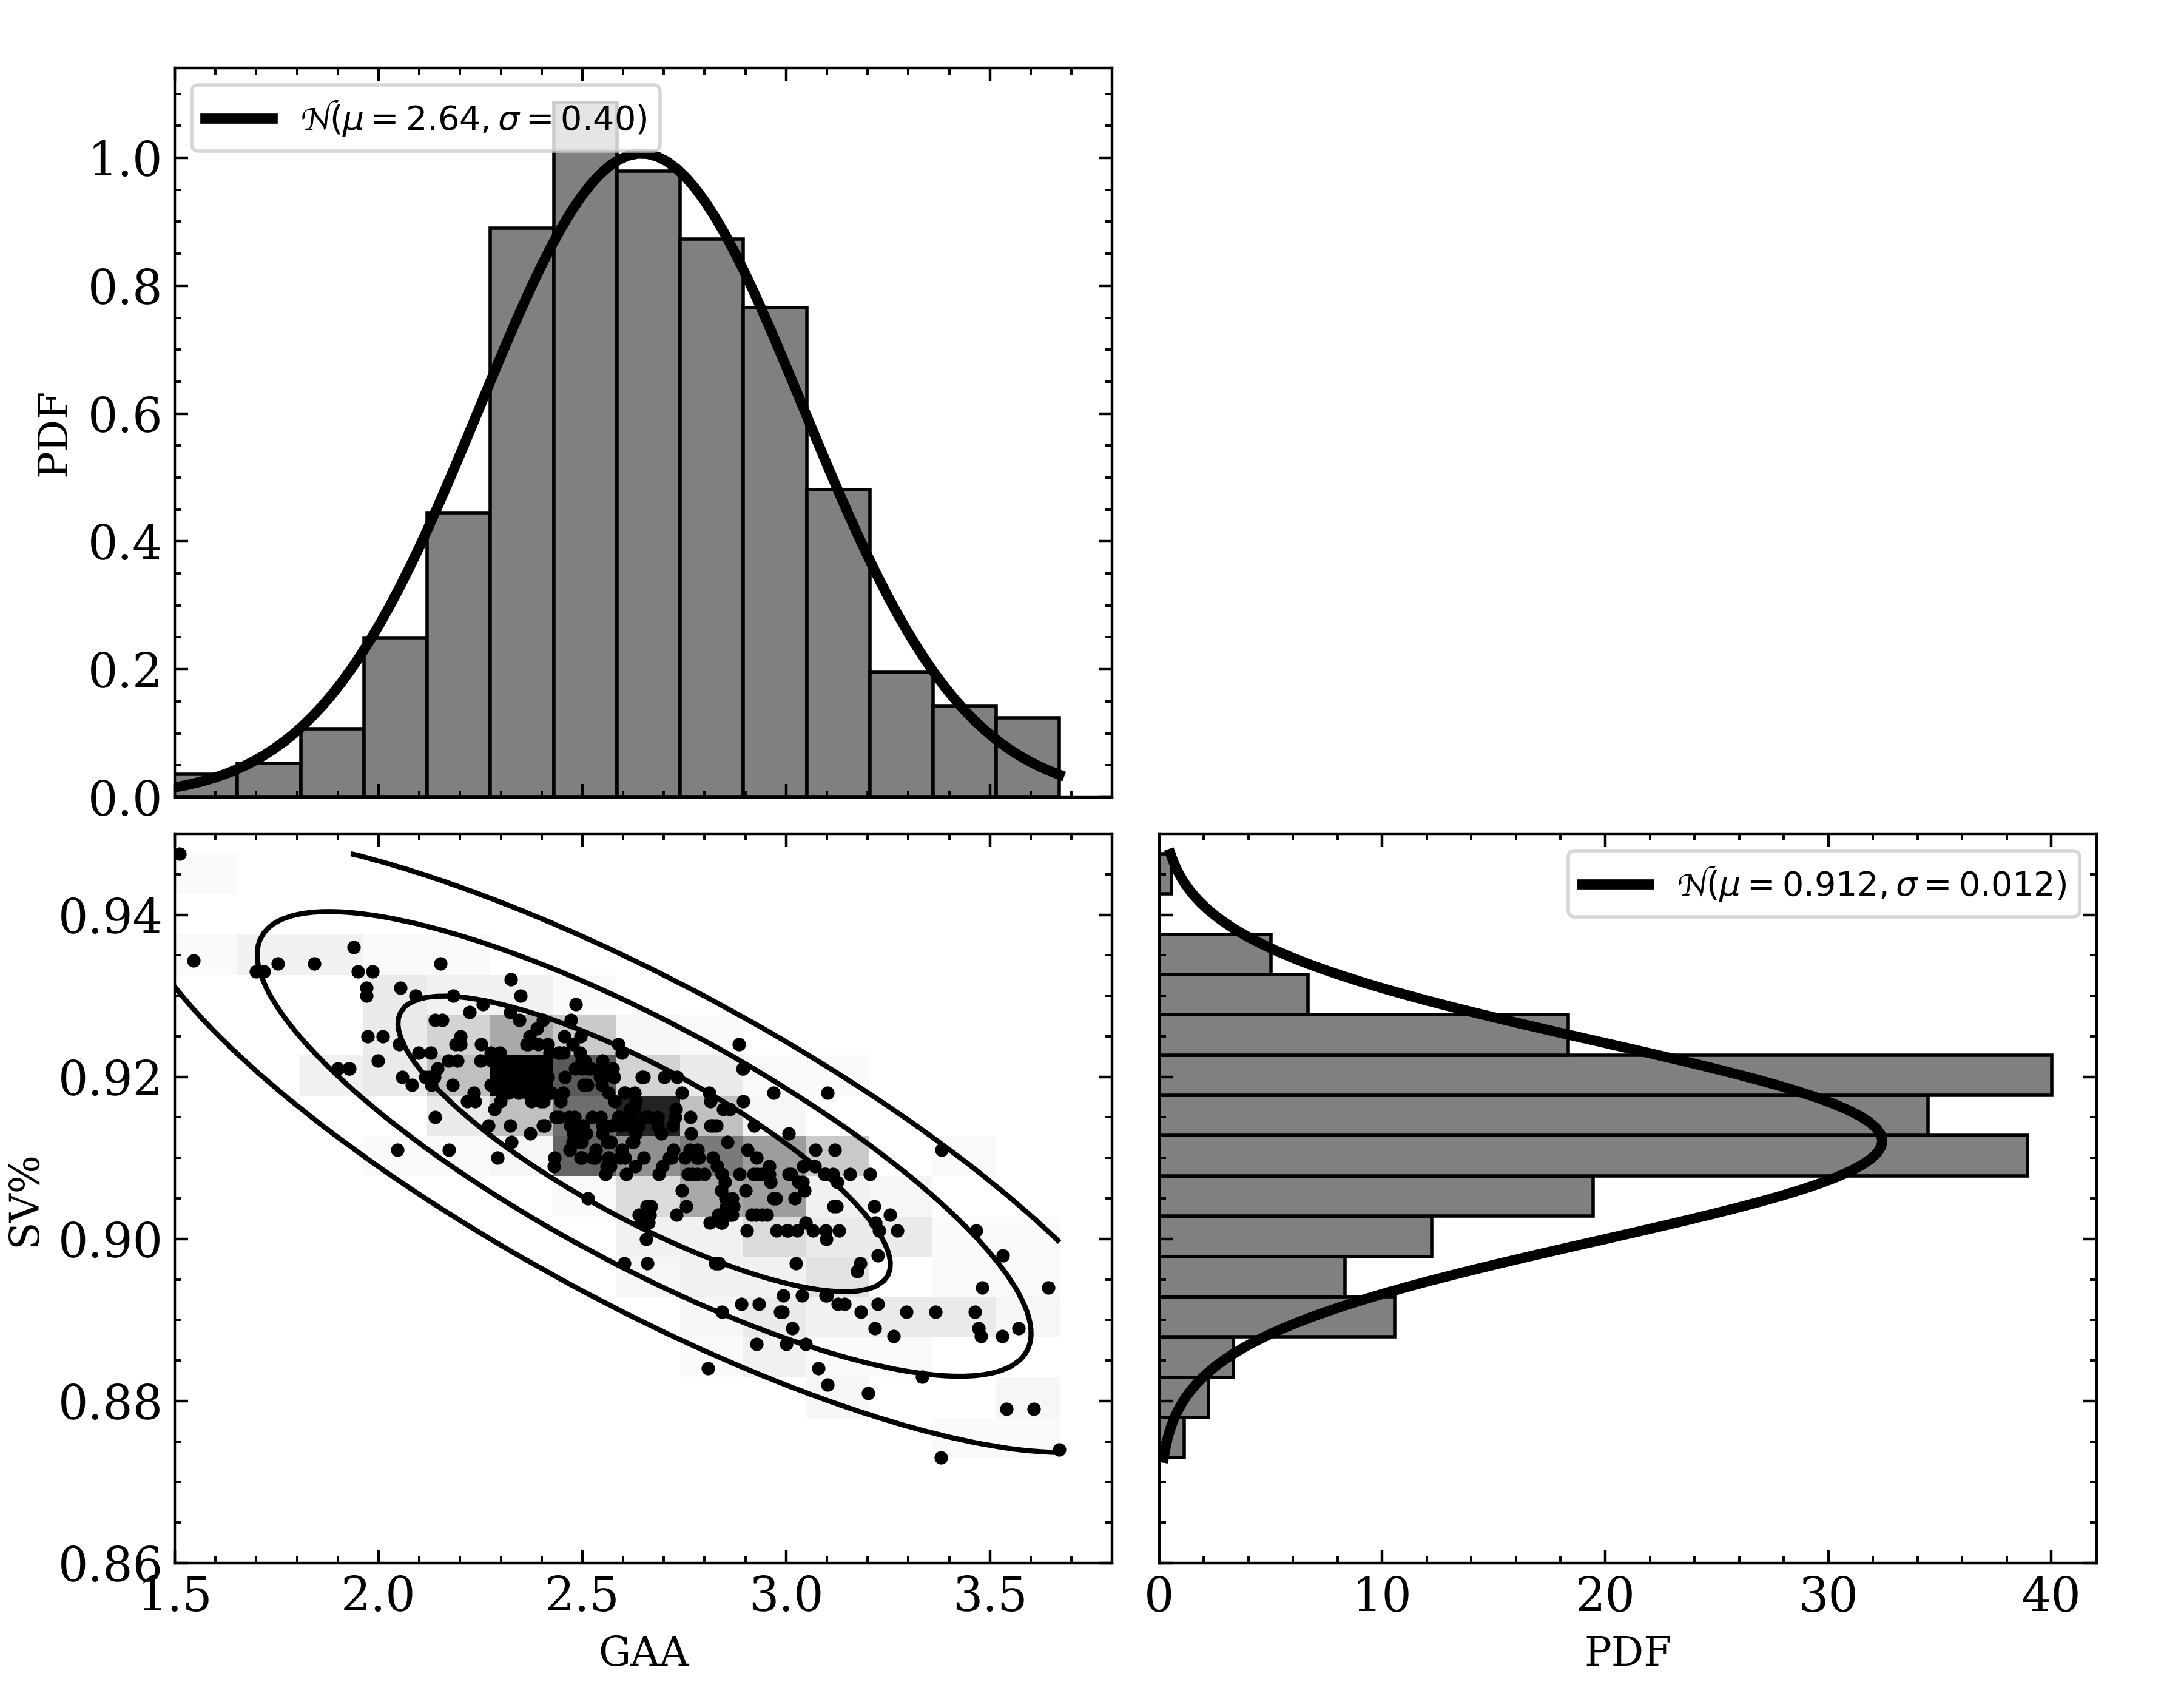
\includegraphics[width=0.9\hsize]{figures/corr_2D_HARTpost_logo_bkgd.png}%
  \hspace{-0.9\hsize}%
  \begin{ocg}{fig:logosoff}{fig:logosoff}{0}%
  \end{ocg}%
  \begin{ocg}{fig:logoson}{fig:logoson}{1}%
   % 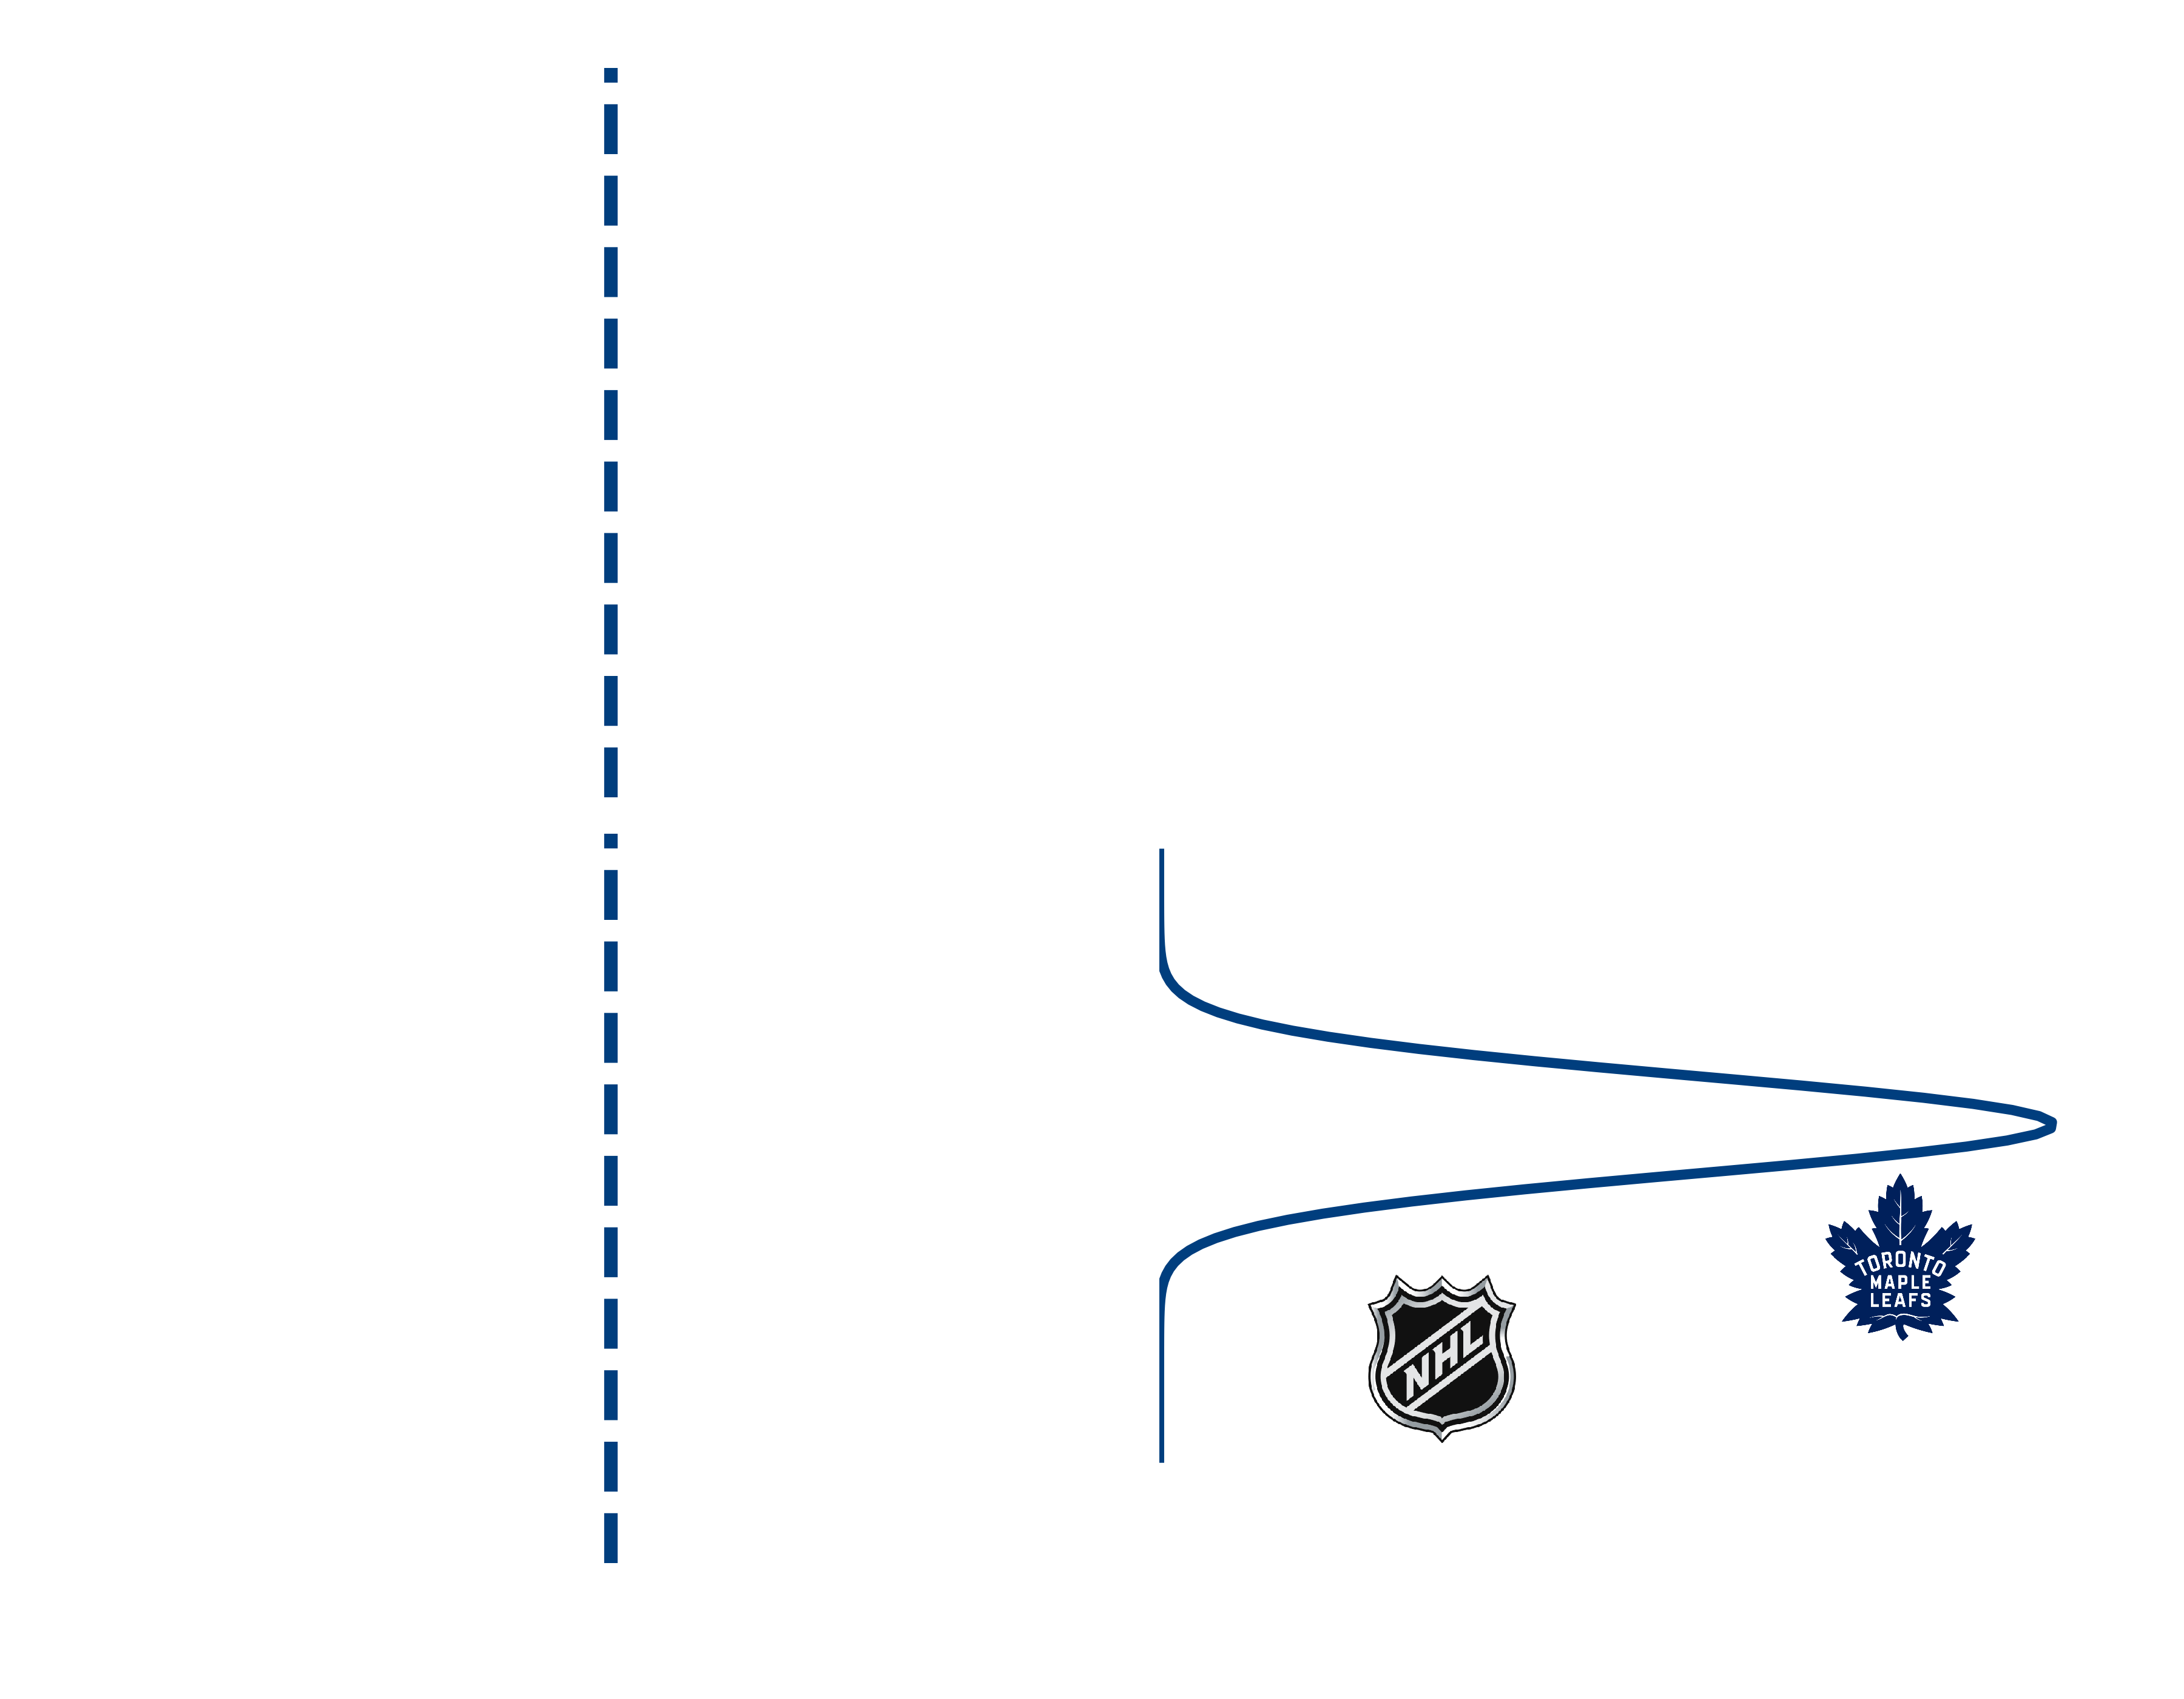
\includegraphics[width=0.9\hsize]{figures/corr_2D_HARTpost_logo_logos.png}%
  \end{ocg}
  \caption[Correlated Gaussian random variables in two dimensions.]
      {The one and two dimensional distributions of the Gaussian random
    variables $GAA$ and $SV$\%.
    The covariance matrix (Eq.~\ref{eq:Kcorr}) has negative off-diagonal
    elements describing the degree of anti-correlation between the two
    variables; a property which is largely discernable from their joint
    distribution as high values of the $SV$\% tend to correspond to a lower
    $GAA$. The correlation can be used to inform the value of one variable given a
    measurement of the other. This is demonstrated as the measured $GAA$ 
    for the Toronto Maple Leafs' goaltender 
    \ToggleLayer{fig:logoson,fig:logosoff}{\protect\cdbox{(vertical dashed line)}}
    provides some
    additional information on the correpsonding $SV$\% whose posterior given the
    measured $GAA$ is more tightly constrained than the $SV$\% distribution for
    the entire NHL.}
  \label{fig:corr2d}
\end{figure}

The fact that the two variables are
correlated implies that knowledge of one variable provides some additional constraining
power on the value of the second. This demonstrated in Fig.~\ref{fig:corr2d}
wherein we measure the value of the $GAA$ for the Toronto Maple Leafs' goaltender
to be 2.57 goals per game. Not bad. Not great, but not bad. By measuring
this value we can establish a posterior distribution on Freddie's corresponding
$SV$\% given his $GAA$: $p(SV\%|GAA=2.57)$. Because the variables are dependent
on each other according to Eq.~\ref{eq:Kcorr}, this posterior distribution is
narrower (i.e. more precise) than the full $SV$\% distribution. Indeed this is
evidenced in the lower right panel of Fig.~\ref{fig:corr2d} which compares the
two $SV$\% distributions and reveals that the dispersion in $p(SV\%|GAA=2.57)$
has approximately half of the dispersion as the full $SV$\% distribution. The degree
of improvement in the predictive distribution of $X_2$ given $X_1$ is dependent
on how strongly correlated the two variables are. \\

\subsection{The $k$-dimensional Gaussian distribution}
So far we have considered a pair of correlated Gaussian random variables whose
PDF is given in Eq.~\ref{eq:gauss2d} for $k=2$. Next we want to extend the multivariate
Gaussian distribution to arbitrarily large $k$ and visualize that distribution which
cannot be done with the conventional contour-based visualization
(Figs.~\ref{fig:uncorr2d} \&~\ref{fig:corr2d}) beyond two dimensions. To resolve this
restriction we now adopt an alternative visualization of a multivariate Gaussian
dicstribution which I call the linear representation which is depicted in
Fig.~\ref{fig:linrep} alongside the conventional representation. Fig.~\ref{fig:linrep}
depicts a finite number of samples from the two dimensional Gaussian distribution shown
in Fig.~\ref{fig:corr2d} in both representations. \\

Each identically coloured line in the
linear representation depicts the values of the scaled $GAA$ and the $SV$\%\footnote{Note
  that the $GAA$ and $SV$\% are scaled to a common unit such that they span roughly
  the same region of the y-axis in the Fig.~\ref{fig:linrep} linear representation.
  The scaling is also such that the correlation between the scaled $GAA$ and $SV$\% is
  now positive (i.e. not anit-correlated).} for a single
sample from their joint distribution. Furthermore the correlation between the two variables,
which we now insist be a positive correlation, is qualitatively apparent as a small value
of the scaled $GAA$ often corresponds to a low value of the scaled $SV$\%. If the two
variables were weakly correlated then we would expect more corssing of curves in the
linear representation then is seen in Fig.~\ref{fig:linrep}. What's more is that the
distribution of values in the vertial direction for each variable is indicative of its
mean and uncertainty. \\

\begin{figure}
  \centering
  %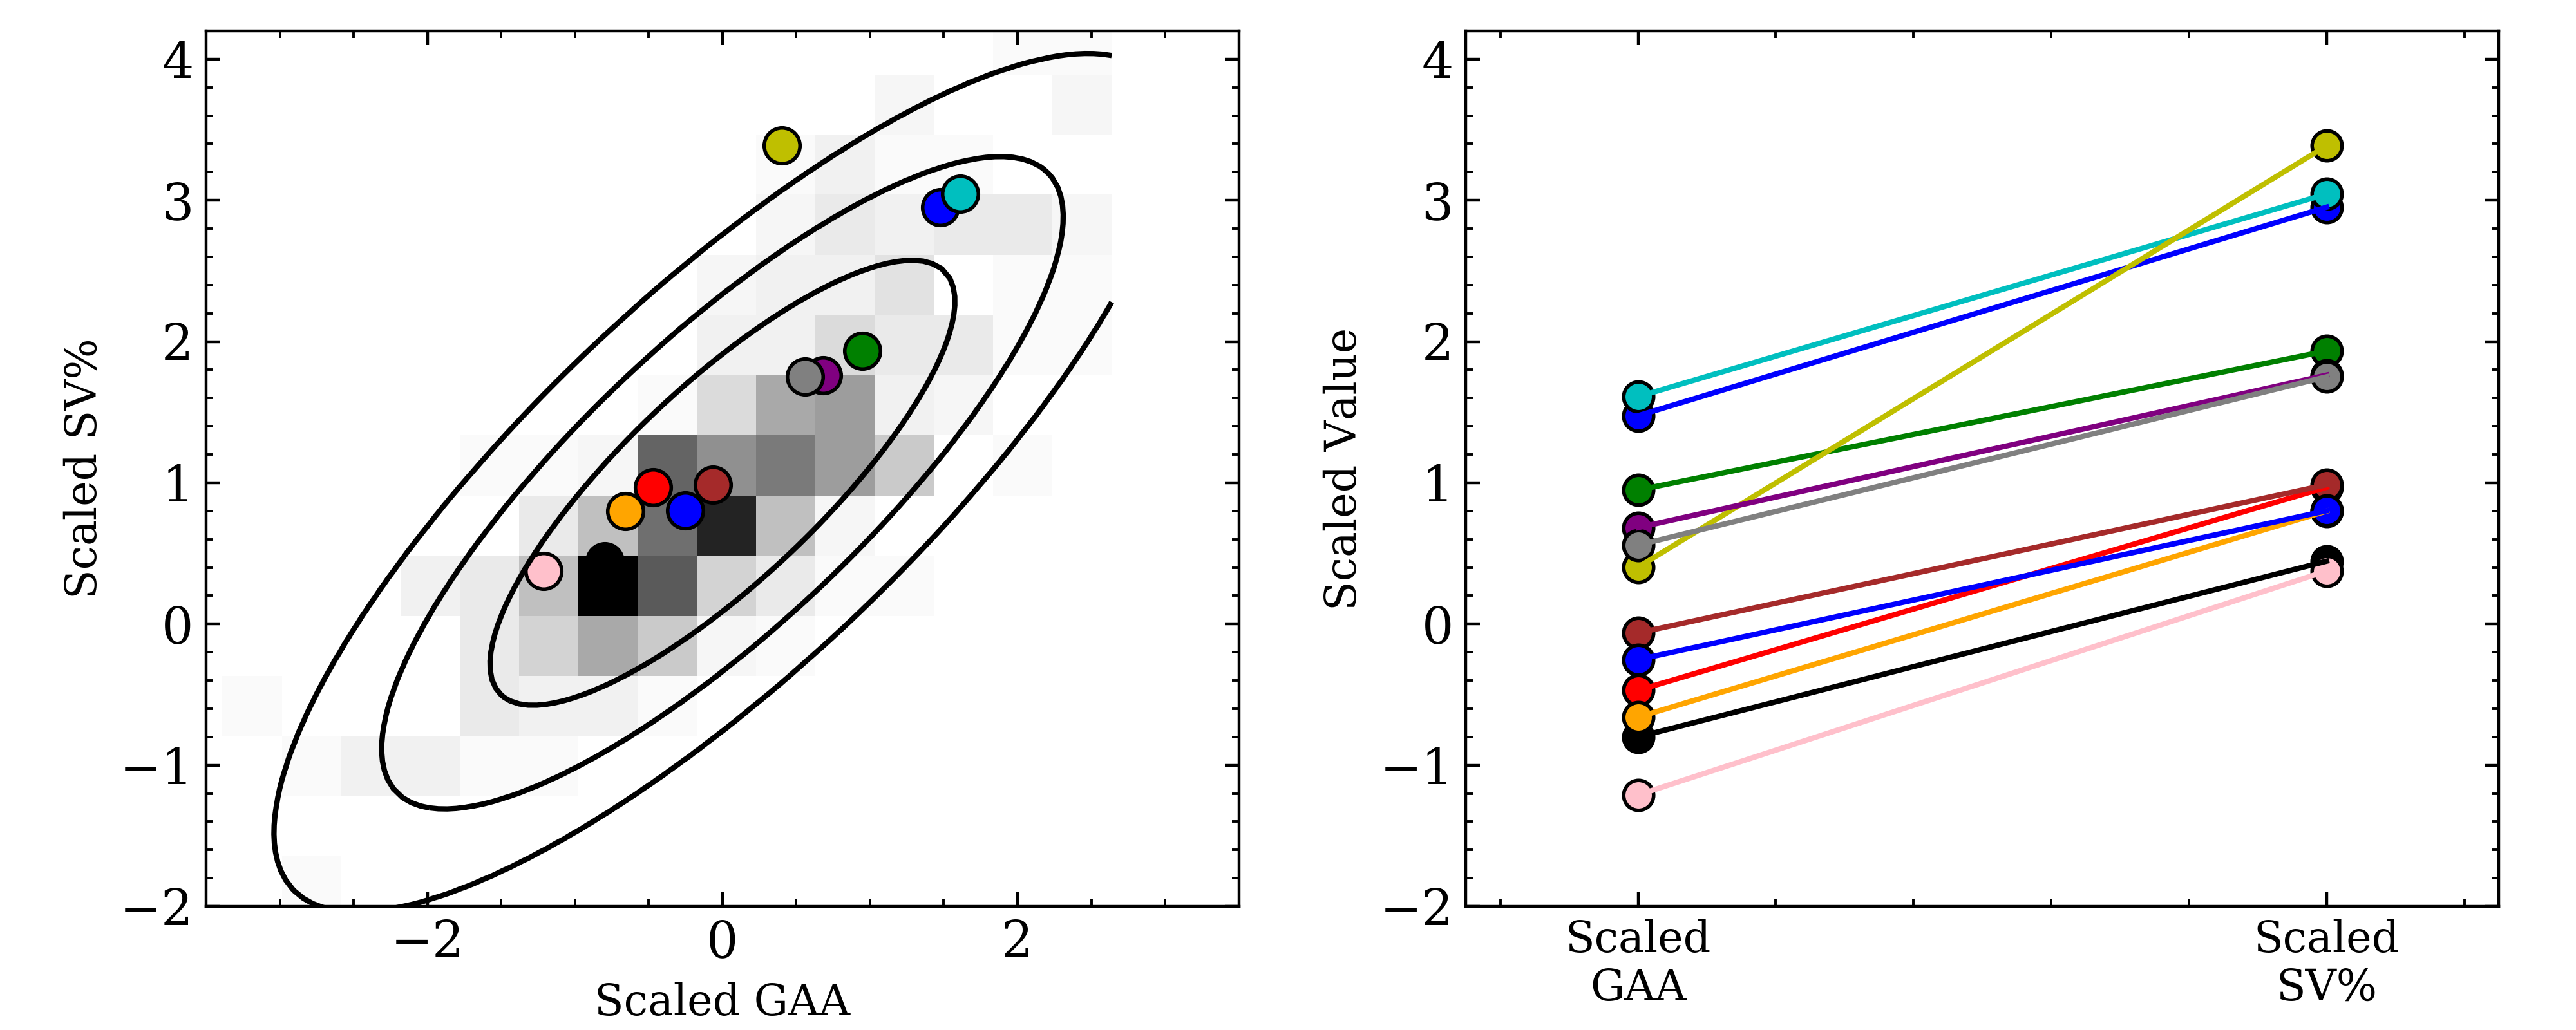
\includegraphics[width=\hsize]{figures/linearrep_v1.png}
  \caption[Linear representation of Gaussian random varaibles in two dimensions.]
          {Visual comparison of samples from the two-dimensional Gaussian distribution
            depicted in the
            conventional way (left panel) and in the new linear representation (right
            panel). The $GAA$ and $SV$\% variables are scaled to a common unit with a
            positive correlation and offset for clarity.}
  \label{fig:linrep}
\end{figure}


The benefit of adopting the new linear representation is that it can be extended to
arbitrarily large dimensions. Fig.~\ref{fig:linrepv2} depicts the linear representation
of an $k=5$ dimensional space which includes three new Gaussian random variables which
are defined to be positively correlated with the scaled $GAA$ and $SV$\%. The left panel
in Fig.~\ref{fig:linrepv2} depicts samples from the five dimensional Gaussian distribution
as well as each variable's mean and $1\sigma$ dispersion. The right panel of
Fig.~\ref{fig:linrepv2} illustrates the effect of how the measurement of one of variables
informs the posteriors of the other variables as a result of their correlation. That is
that when the third variable in Fig.~\ref{fig:linrepv2} is measured and its uncertainty
goes to zero, the posterior distributions on the remaining variables are narrowed. As
more and more variables are measured, constraints on the unmeasured variables would
similarly increase in a way that is quantified by the correlations between the
measured and unmeasured variables.
The notion that the value of an unseen variable can be informed by the measurement
of another, if those variables are correlated, has major implications for
predictive models as we shall see in Sect.~\ref{sect:regression}. \\

\begin{figure}
  \centering
  %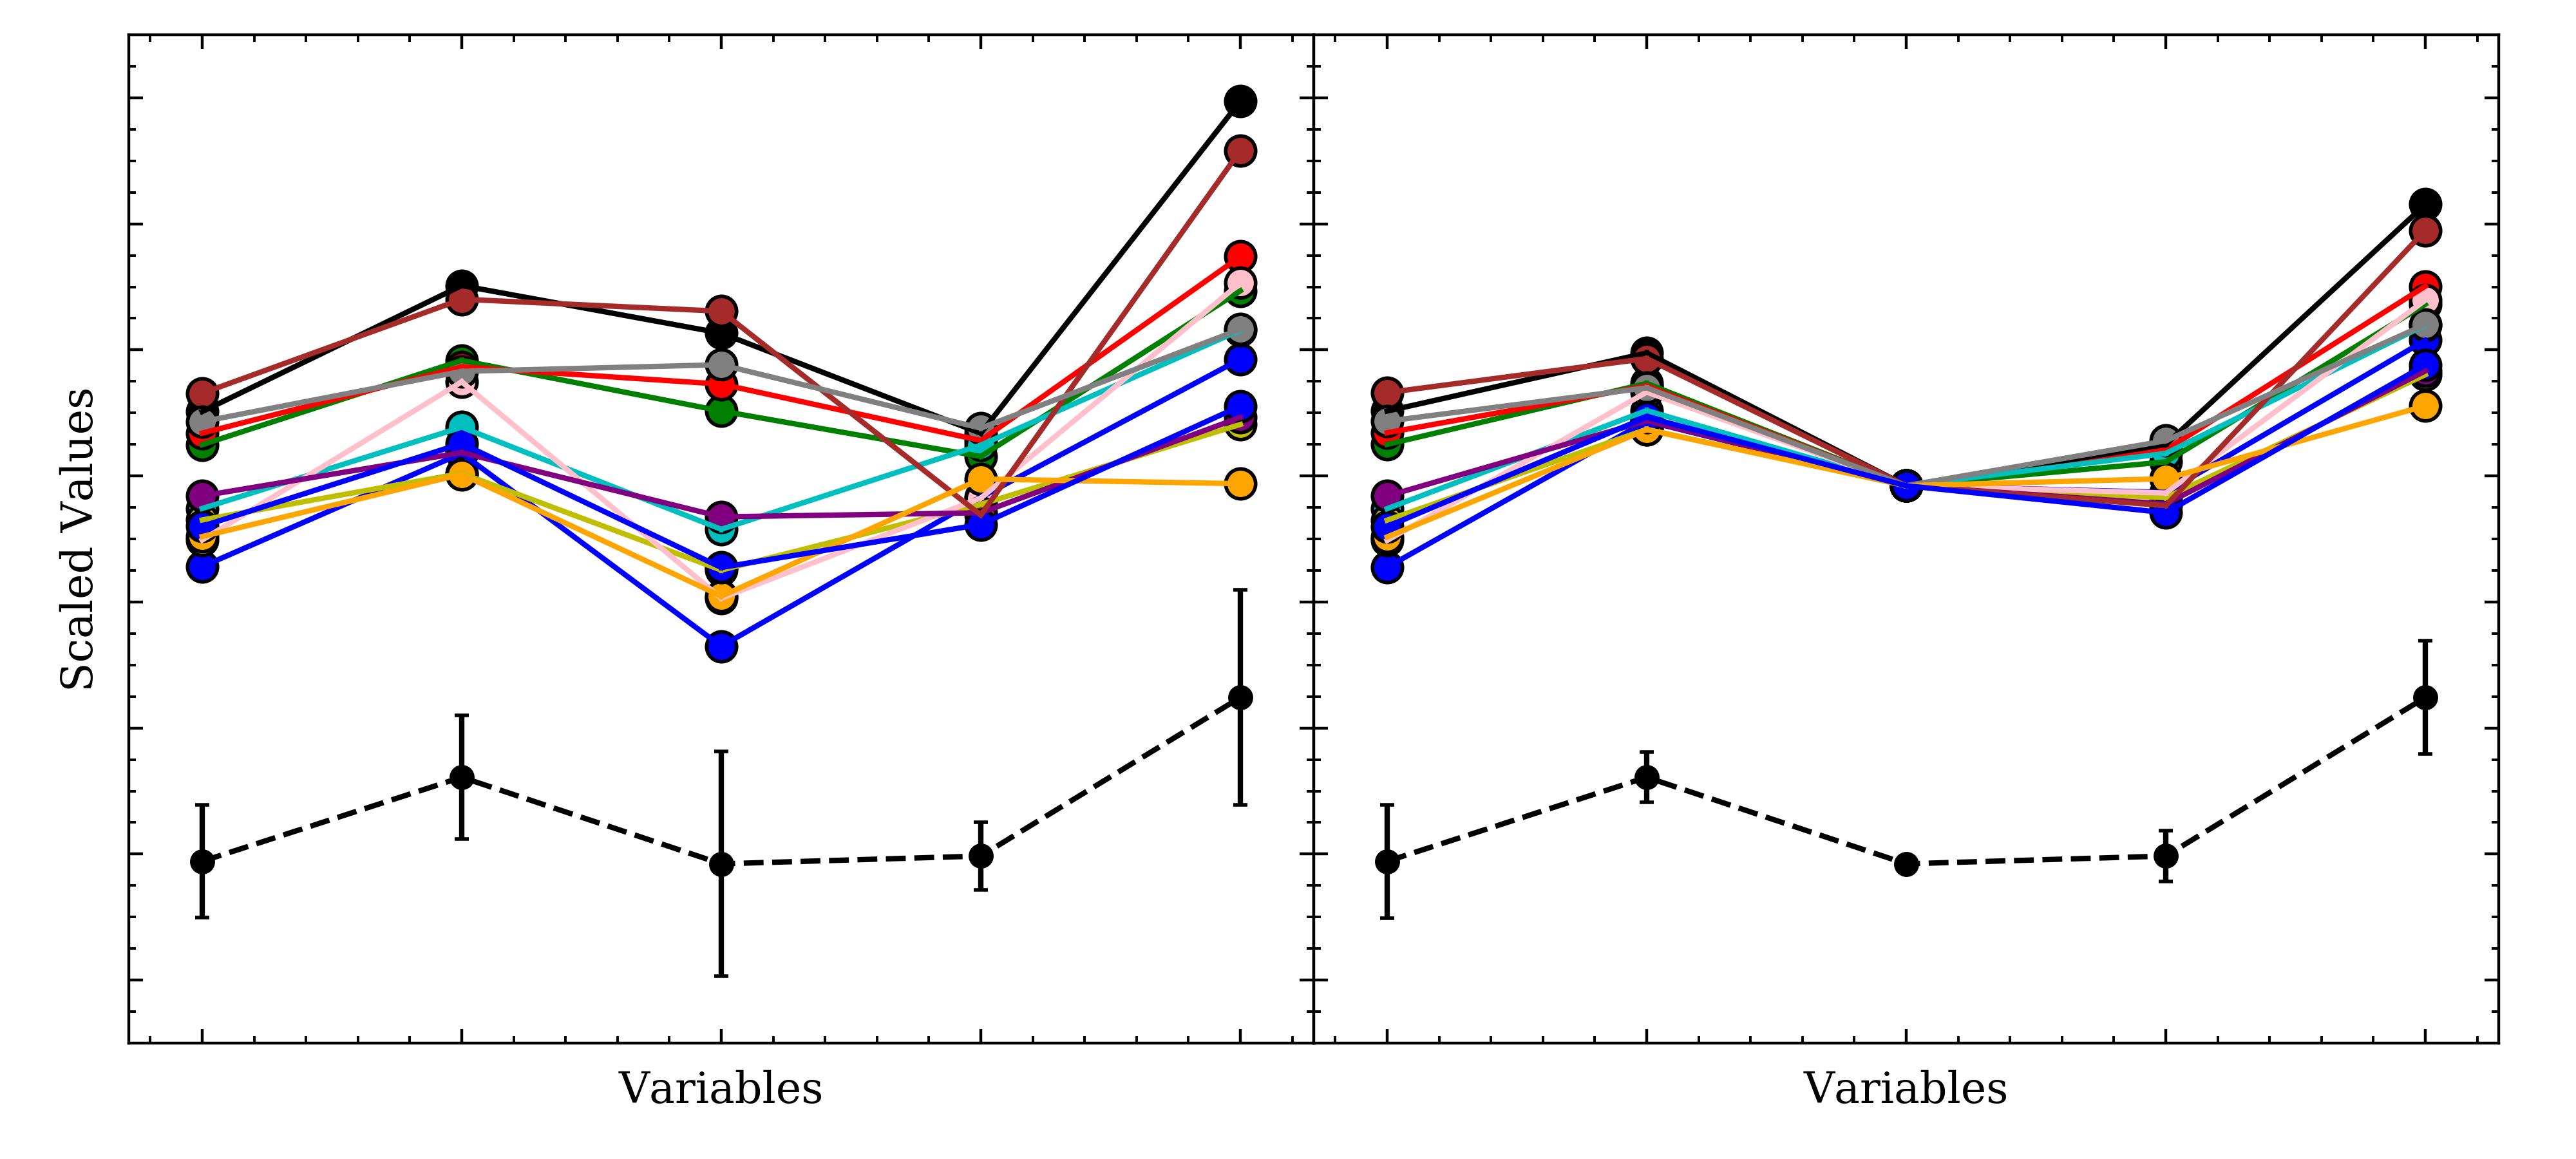
\includegraphics[width=\hsize]{figures/linearrep_v2.png}
  \caption[Linear representation of Gaussian random varaibles in five dimensions.]
          {The linear representation of samples from a five dimensional Gaussian
            distribution with each sample depicted with a particular colour in each
            panel. The mean and $1\sigma$ dispersion of each variable is depicted
            by the offset black markers and error bars. The right panel illustrates
            how the measurement of the third variable constrains the values of the
            remaining variables due to their correlations.}
  \label{fig:linrepv2}
\end{figure}


\subsection{Gaussian process regression modelling} \label{sect:regression}
Upon inspection of Fig.~\ref{fig:linrepv2}, one might imagine changing the ``variables''
axis to and independent variable such as time and the ``scaled values'' axis to an
observable such as stellar RVs. Because RV signals arising from active stars are temporally
correlated as active regions rotate in and out of view of the observer, it is clear that
modelling the correlation between adjacent RV observations could be used to inform
our understanding of the activity signal in a way that is independent of attempting to
model the physical nature of the signal. \\

Indeed one dimension Gaussian process (GP) regression models are a convenient method to model
correlations between observations in a semi-parametric way. In particular, GPs provide a
flexiable framework to perform Bayesian inference on functions. Their flexibility stems from
their semi-parametric nature which makes them well-suited to modelling stochastic processes
like stellar activity which lack a determinstic functional form. GP regression works to model
the covariance between data points simultanously with determinstic components such as planets
on keplerian orbits. Given a parameterization of the data covariance structure, the GP is
by definition a multivariate Gaussian distribution with a well-defined mean function and
variance which represent our model of the correlated observables and its uncertainty
\citep{rasmussen05}. \\

\subsubsection{Covariance kernel functions}
Modelling of temporally correlated stellar activity with a GP regression model first requires
a parameterization of the data covariance. This parameterization of an analytical
covariance kernel through a small set of hyperparameters\footnote{``Small''
  relative to the number of RV measurements.} is why GP regression models are often referred to
as semi-parametric. The covariance matrix of the GP is written in terms of the covariance kernel
function $k(t,t')$ as

\begin{equation}
  \mathbf{K}_{ij} = k(t_i,t_j) + \delta_{ij} \sqrt{\sigma_{\text{RV}}^2(t_i) + s^2} 
\label{eq:Kmat}
\end{equation}

\noindent where the indices run up to the number of RV measurements (i.e. $i,j=1,\dots,$\nrv{)}.
Because of the Dirac delta function $\delta_{ij}$ in Eq.~\ref{eq:Kmat}, the 
diagonal of the covariance matrix $\mathbf{K}$ includes contributions directly from the
RV measurement uncertainties \sigRV{} plus an additive scalar jitter $s$ designed to absorb excess
white noise from systematics or from other temporally independent noise sources. \\

A number of covariance kernels which have been proposed
for the treatment of stellar RV activity are summarized below. Their corresponding covariance
matrices are also shown in Fig.~\ref{fig:matrices}. \\

\begin{figure}
  \centering
  %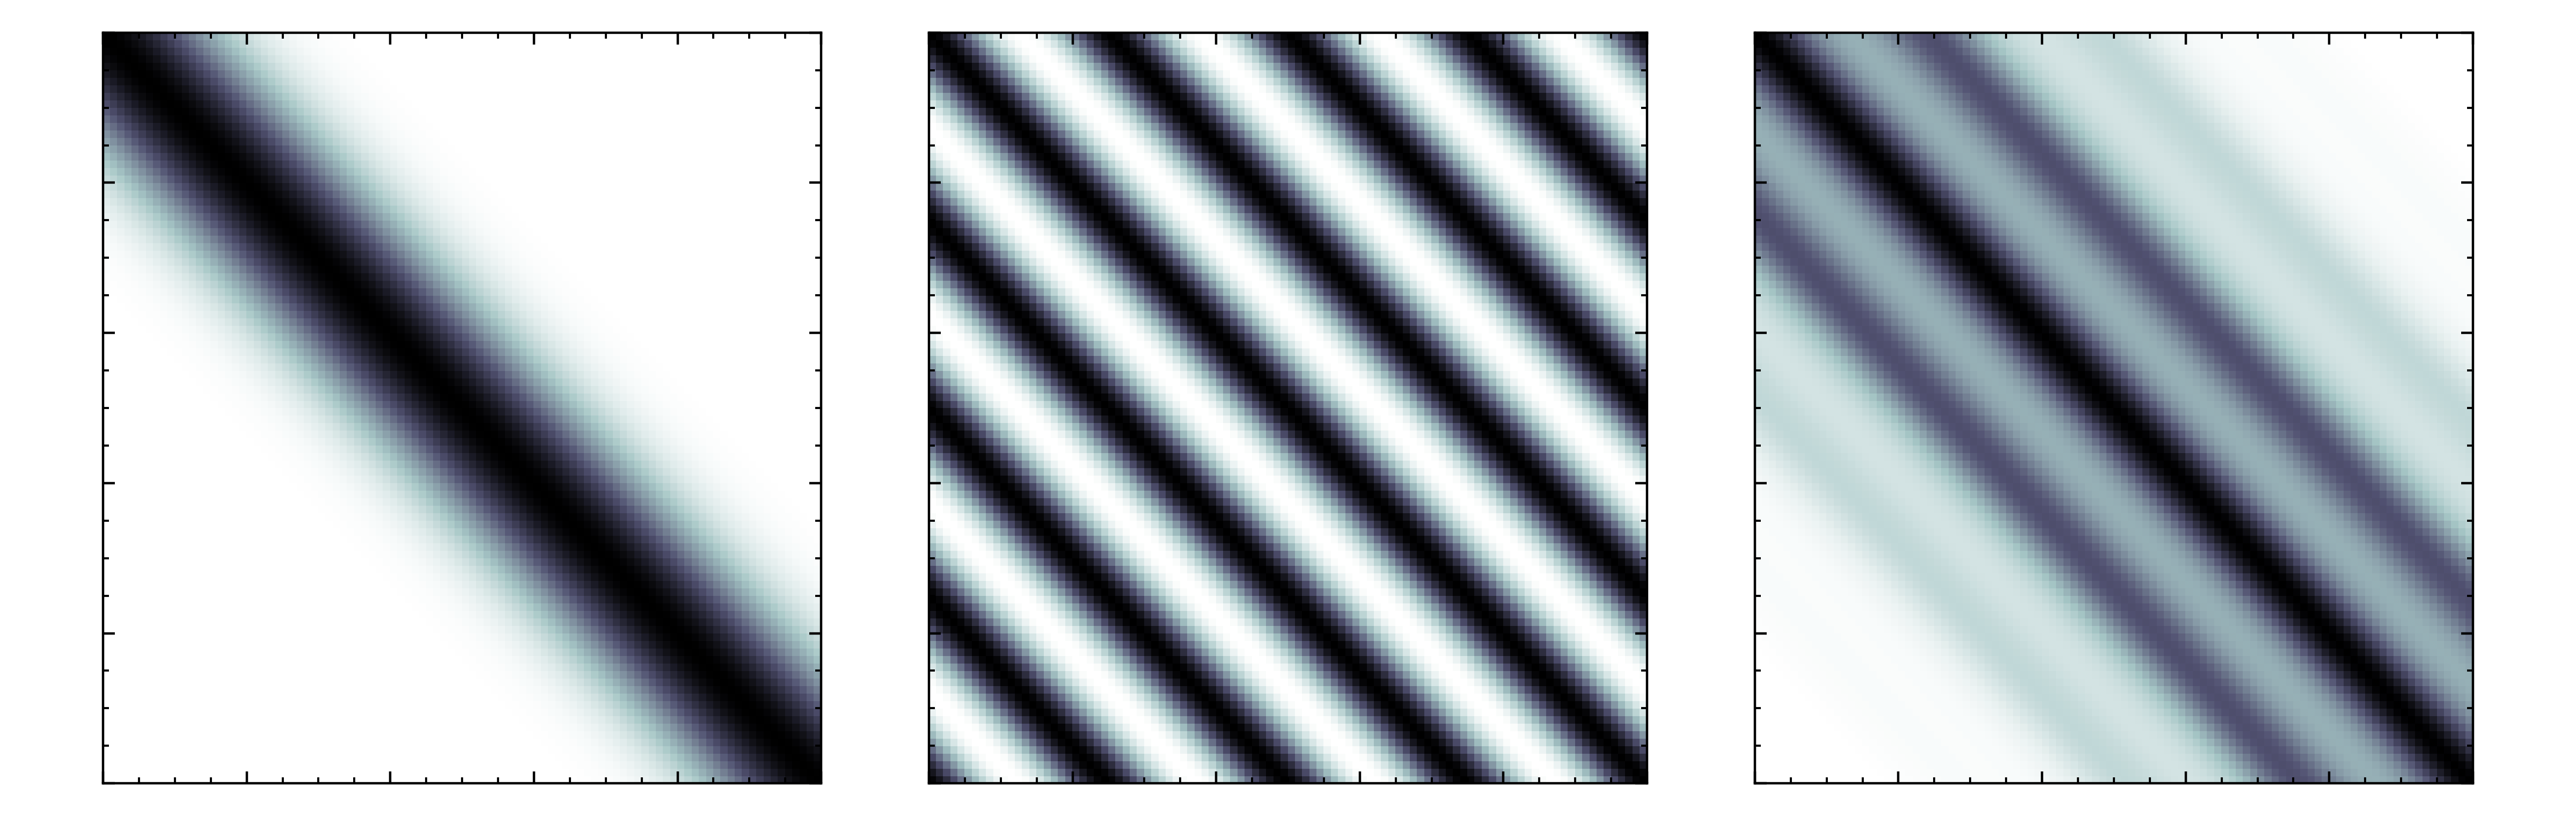
\includegraphics[width=\hsize]{figures/gpmatrices.png}
  \caption[Example of covariance matrices.]
          {Examples of covariance matrices with a squared exponential covariance kernel (left),
            a periodic covariance kernel (middle), and a quasi-periodic covariance kernel (right).
            In this example the exponential timescale exceeds the periodic timescale such that the
            nearly periodic nature of the covariance is still discernable for points closely separated
          in time (i.e. near the matrix diagonal).}
          \label{fig:matrices}
\end{figure}

\emph{Squared exponential}: 

\begin{equation}
  k_{\text{SE}}(t_i,t_j) = a^2 \exp{\left[ -\frac{(t_i-t_j)^2}{2\lambda^2} \right]},
\end{equation}

\noindent has two hyperparameters. Namely, the covariance amplitude $a$ in units of the observable,
and an exponential timescale $\lambda$ describing how much time is required for measurements to
effectively forget previous values. With this covariance kernel measurements made closely in time
are more highly correlated than well separated measurements and the degree of correlation for a
given time separation will be larger for smaller $\lambda$. \\

\emph{Periodic}:

\begin{equation}
  k_{\text{P}}(t_i,t_j) = a^2 \exp{\left[ -\Gamma \sin^2{\left( \frac{\pi |t_i-t_j|}{P} \right)} \right]},
\end{equation}

\noindent has three hyperparameters including the familiar covariance amplitude $a$. The periodic kernel
also contains a coherence parameter $\Gamma$ and a periodic timescale $P$ within the sinusoidal term.
With this covariance kernel measurements that are separated by an integer number of $P$ will be highly
correlated. \\

\emph{Quasi-periodic}:

\begin{equation}
  k_{\text{QP}}(t_i,t_j) = a^2 \exp{\left[ -\frac{(t_i-t_j)^2}{2\lambda^2} -\Gamma
      \sin^2{\left( \frac{\pi |t_i-t_j|}{P} \right)} \right]},
\end{equation}

\noindent is the product of the squared exponential and periodic covariance kernels and therefore
contains all four unique hyperparameters amongst the two kernels. \\

Stellar activity on M dwarfs
is dominated by active regions\citep{lindegren03}\footnote{And sometimes flares but those
  occur on short timescales such that they rarely affect low cadence RV osbervations for almost
  all but the most active flare stars.} and the resulting RV signals evolve in a manner that
is easy to understand qualitatively. Namely, we can expect a periodic component to the
RV correlations because active regions rotate in and out of view at the stellar rotation period
although the periodicity of the correlations need not be at \prot{} and may instead appear
at a low order harmonic of \prot{} such as in the case of rapidly rotating spotted stars 
(see Sect.~\ref{sect:ffp}). But in addition to these periodic variations, we can expect activity
arising from active regions to not be stricitly periodic because of active region evolution
in terms of their sizes, temperatures, and spatial distributions. Thus we
have a physical justification for the adaption of a
quasi-periodic covairance kernel as it includes the squared exponential term
whose timescale can be thought of a characterizing active region lifetimes. \\

The optimiziation of the quasi-periodic covariance kernel over competing kernel functions
was demonstrated by \cite{grunblatt15} on the active Sun-like star Kepler-78. However, it
should be noted that due to the semi-parametric nature of GP regression models, the exact
choice of kernel and/or the exact values of its hyperparameters often do not matter as
much as one might think. Fig.~\ref{fig:exactgp} illustrates this notion by modelling a
set of synthetic data points with each of the three covariance functions defined above.
The synthetic data are generated by a sinusoidal function plus a decreasing linear trend. 
Each GP does a qualitatively similar job at modelling the data and with comparable $1\sigma$
uncertainties. \\

Also depicted in Fig.~\ref{fig:exactgp} is the effect of varying the hyperparameters of
a quasi-periodic GP regression model to the same sythetic data. The first curve depicts
the resulting GP model using the approximate optimized hyperparameters with a periodic
timescale approximately equal to the injected timescale of 50 (arbitrary units). The second
GP model has the same periodic timescale but whose exponential timescale is greater by nearly
three orders of magnitude. Despite this the resulting mean GP appears to continue to be a good
fit to the data. The final GP model reverts back to the optimized exponential timescale but
decreases the periodic timescale from 50 to 20. The effect of a shorter periodic timescale
is only apparent in the regions between data points as the resulting GP again appears to do
a qualitatively similar job at modelling the data depsite having widely varying hyperparameters.


\subsubsection{Hyperparameter estimation}
Determination of the GP hyperparameters $\boldsymbol{\Theta}$ for a given covariance kernel is
done by first specifying a mean model $\boldsymbol{\mu}$ which itself is parameterized by
a set of model parameters $\boldsymbol{\theta}$. In the case of modelling RVs the mean model
might represent our planet model whose keplerian orbital parameters are what we are interested
in measuring as the GP is used to model the correlated RV residuals arising from stellar
activity. The residual vector is written as $\mathbf{r} = \mathbf{y} - \boldsymbol{\mu}$
where $\mathbf{y}$ is the vector of \nrv{} measurements. 
To estimate all model parameters, including the GP hyperparameters and mean model
parameters (i.e. $\boldsymbol{\Psi} = \boldsymbol{\Theta} \cup \boldsymbol{\theta}$),
we sample their joint posterior according to Bayes theorem

\begin{equation}
  p(\boldsymbol{\Psi}|\mathbf{y}) \propto \mathcal{L}(\mathbf{y}|\boldsymbol{\Psi}) \cdot
  \Pi(\boldsymbol{\Psi})
  \label{eq:bayess}
\end{equation}

\noindent where

\begin{equation}
  \mathcal{L}(\mathbf{y}|\boldsymbol{\Psi}) =
  -\frac{1}{2} \left( \mathbf{r}^{\text{T}} \mathbf{K}^{-1} \mathbf{r} +
  \ln{\text{det}\mathbf{K}} + N_{\text{RV}} \ln{2\pi} \right)
\end{equation}

\noindent is the logarithmic likelihood function given the set of model parameters
$\boldsymbol{\Psi}$ and $\Pi(\boldsymbol{\Psi})$ represents our prior on
the model parameters. When estimating the GP hyperarameters in practice we
often sample the logarithmic hyperparameters and adopt broad log uniform priors
unless otherwise stated. Note that in Eq.~\ref{eq:bayess}
we have neglected the normalization factor which is not required
for the purpose of parameter estimation. \\

Sampling of the $\boldsymbol{\Psi}$ posteriors is done using MCMC. In this way, our
uncertainties in the keplerian model parameters $\boldsymbol{\theta}$,
that are of interest for studying planets, are marginalized over our uncertainties in
the GP hyperparameters $\boldsymbol{\Theta}$. The exact details of
our MCMC implementation and strategies are discussed in subsequent chapters
as necessary. After sampling the $\boldsymbol{\Psi}$ posteriors, the values of the
hyperparameters are obtained from the maximum a-posteriori point estimates of those
posteriors which in turn are used to define our GP activity model.

\subsubsection{Model inference}
From the set of hyperparameters $\boldsymbol{\Theta}$,
we define a unique GP prior distribution. From this distribution we can sample
functions or construct a predictive distribution
conditioned on the data $\mathbf{y}(\mathbf{t})$ and evaulated at some unseen
epochs $\mathbf{t}^*$. Function predictions from such a predictive distribution is
historically known as kriging. The mean function and standard deviation of the
predictive distribution are

\begin{equation}
  \boldsymbol{\mu}(\mathbf{t}^*) = \mathbf{K}(\mathbf{t}^*,\mathbf{t}) \cdot
  \mathbf{K}(\mathbf{t},\mathbf{t})^{-1} \cdot \mathbf{y}(\mathbf{t}),
  \label{eq:gpmu}
\end{equation}

\noindent and

\begin{equation}
  \boldsymbol{\sigma}(\mathbf{t}) = \mathbf{K}(\mathbf{t}^*,\mathbf{t}^*) -
  \mathbf{K}(\mathbf{t}^*,\mathbf{t}) \cdot \mathbf{K}(\mathbf{t},\mathbf{t})^{-1}
  \cdot \mathbf{K}(\mathbf{t}^*,\mathbf{t})^{\text{T}}.
  \label{eq:gpsig}
\end{equation}

Figs.~\ref{fig:gpsamples} and~\ref{fig:gpsamplespred} depict samples from a
quasi-periodic GP prior and predictive distributions respectively. The latter is
conditioned on an set of ten synthetic data points and whose mean function and
standard deviation are computed using Eqs.~\ref{eq:gpmu} and~\ref{eq:gpsig}. When
modelling RV activity with a GP whose hyperparameters $\boldsymbol{\Theta}$ have
been derived from MCMC, we take the ``best-fit'' of that multivariate Gaussian, namely
its mean function, to be our activity model similarly to how maximum a-posteriori
point estimates of keplerian orbital parameters are used to compute a ``best-fit''
planet model. \\

\begin{figure}
  \centering
  %\animategraphics[width=\textwidth,controls,loop]{5}{figures/GPsample_}{0}{1}
  \caption[Samples from a quasi-periodic Gaussian process prior distribution.]
          {Continuous samples from a quasi-periodic Gaussian process prior distribution.
            A discontinuity in the sampling occurs after 50 frames. This animation was
            generated using code written by Jo\~ao
            Faria (\url{https://joaofaria.space/blog/continuous-samples}).}
  \label{fig:gpsamples}
\end{figure}

\begin{figure}
  \centering
  %\animategraphics[width=\textwidth,controls,loop]{5}{figures/GPsample_pred_}{0}{49}
  \caption[Samples from a quasi-periodic Gaussian process predictive distribution.]
          {Independent samples from a quasi-periodic Gaussian process predictive distribution
            conditioned on ten synthetic data points. The mean function and
            $1\sigma$ standard deviation are depicted as the dashed black curve and surrounding
          shaded region respectively.}
  \label{fig:gpsamplespred}
\end{figure}


\subsection{Demonstrating the effectiveness of a GP activity model: a toy model}



\begin{figure}
  \centering
  %\includegraphics[width=0.8\hsize]{figures/}
  \caption{Comparison of injected RV activity to the GP activity model}
  \label{fig:GPperformance}
\end{figure}


ribas18: GP can absorb some planet signal


GP codes:
\texttt{scikit-learn} \citep{sklearn},
\texttt{george} \citep{ambikasaran14,foremanmackey15b},
\texttt{celerite} \citep{foremanmackey17},
\texttt{gpytorch} \citep{gardner18,wang19}.


\section{Point-form Thesis: Stellar Activity Modelling in Radial Velocity
  Time Series}
\begin{itemize}
\renewcommand\labelitemi{--}
\item~\ref{sect:methods} \textbf{An Overview of Techniques for Stellar Activity
Mitigation}: hi \\
\item~\ref{sect:gp} \textbf{Gaussian Process Regression for Non-Parametric
  Activity Modelling}:
\end{itemize}
